\section{Волновые процессы в средах сложной структуры}

\subsection{Объёмные волны}

\subsubsection{Аналитическое решение}

Для изотропного однородного упругого тела уравнения движения можно представить как дифференциальное уравнение в векторной форме:

\begin{equation}
(\lambda+\mu)\nabla{div\vec{u}} + \mu\Delta\vec{u} + \rho(\vec{F}-\frac{\partial^2 u}{\partial t^2}) = 0,
\end{equation}

где $\lambda, \mu$ -- параметры Ламе, $\rho$ -- плотность, $\vec{u}$ -- вектор перемещений, $\vec{F}$ -- объёмная сила.

Рассмотрим безграничную среду и представим массовые силы и поле перемещений в виде:
\begin{eqnarray}
\vec{F} = \nabla\Phi + rot\Psi, \\
\vec{u} = \nabla\phi + rot\psi.
\end{eqnarray}

После подстановки и изменения порядка дифференциальных операторов получаем
\begin{equation}
\nabla[c_1^2\Delta\phi - \frac{\partial^2 \phi}{\partial t^2} + \Phi] + rot[c_2^2\Delta\psi - \frac{\partial^2 \psi}{\partial t^2} + \Psi],
\end{equation}

где 
\begin{eqnarray}
c_1^2 = \frac{\lambda+2\mu}{\rho}, \\
c_2^2 = \frac{\mu}{\rho}.
\end{eqnarray}

Таким образом, векторное поле $\vec{u}$ является решением уравнения, если функции $\phi$ и $\psi$ удовлетворяют соотношениям
\begin{eqnarray}
c_1^2\Delta\phi - \frac{\partial^2 \phi}{\partial t^2} = -\Phi, \\
c_2^2\Delta\psi - \frac{\partial^2 \psi}{\partial t^2} = =\Psi.
\end{eqnarray}

Рассмотрим ситуацию, когда $\Psi \equiv 0$, а начальное условия $t = t_0, \phi = 0$. Тогда для определения $\phi$ получается однородное уравнение с нулевыми начальными условиями. Это означает, что $\phi \equiv 0$. Следовательно, в волне, описываемой такими условиями, не происходит вращения частиц среды, т.е. каждая из них движется поступательно. Такие волны называются продольными.

Аналогично, для $\Phi \equiv 0$ мы получим волны, для которых объемное расширение равно нулю. Такие волны называются поперечными или волнами сдвига. Заметим, что при распространении продольные волны не генерируют поперечных, и наоборот. Скорости распространения их фронтов -- $c_1$ и $c_2$ соответственно.


\subsubsection{Расчёт продольной волны (P-волны)}
Пусть плоская P-волна в среде распространяется вдоль оси z. В этом случае аналитическое решение даЁт следующие соотношения на параметры волны:
\begin{itemize}
\item $v_z=-f(z)\sqrt{\frac{\lambda+2\mu}{\rho}}=C_p$;
\item $v_x=v_y=0$;
\item $\sigma_{zz}=f(z)(\lambda+2\mu)$;
\item $\sigma_{xx}=\sigma_{yy}=f(z)\lambda$;
\item $\sigma_{ij}=0$ для $i \neq j$.
\end{itemize}
Здесь $f(z)$ - произвольная функция, зависящая только от z и задающая форму волны.
Для расчёта распространения P-волны в кубе были использованы следующие безразмерные параметры: 
\begin{itemize}
\item $\lambda=70000$;
\item $\mu=10000$;
\item $\rho=1$.
\end{itemize}
На графиках (см. рис. \ref{pic:p_wave}) представлены результаты численного расчёта. Получено совпадение параметров волны с аналитическим решением:
\begin{itemize}
\item $v_z=C_p=300$;
\item $\frac{\sigma_{zz}}{\sigma_{xx}}=\frac{\sigma_{zz}}{\sigma_{yy}}=\frac{\lambda+2\mu}{\lambda}=\frac{9}{7}$.
\end{itemize}

\begin{figure}[htp]
\begin{subfigure}[b]{0.5\textwidth}
\centering
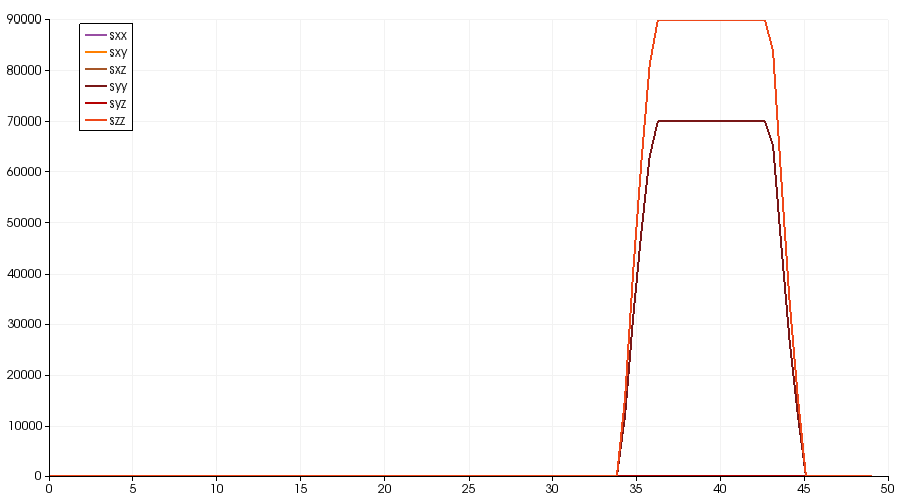
\includegraphics[width=0.8\textwidth]{png/p-wave-test/s/0001.png}
\caption{1-й временной слой}
\end{subfigure}
\begin{subfigure}[b]{0.5\textwidth}
\centering
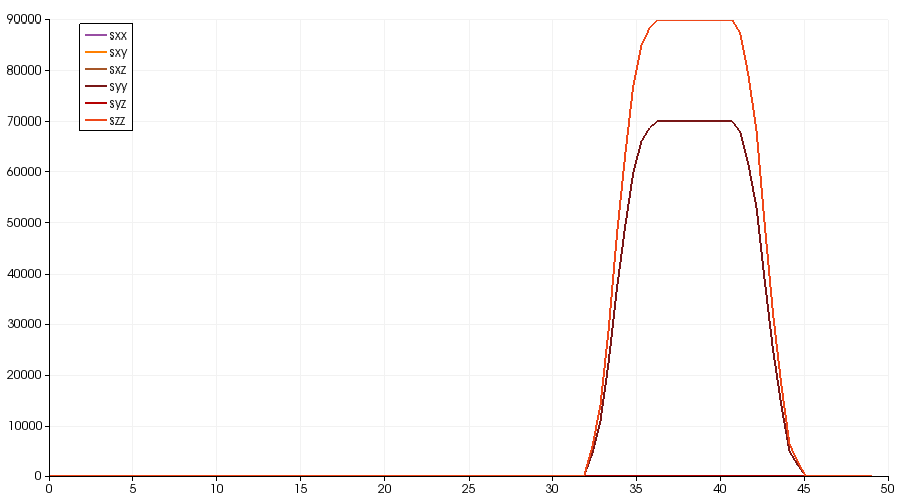
\includegraphics[width=0.8\textwidth]{png/p-wave-test/s/0003.png}
\caption{3-й временной слой}
\end{subfigure}
\begin{subfigure}[b]{0.5\textwidth}
\centering
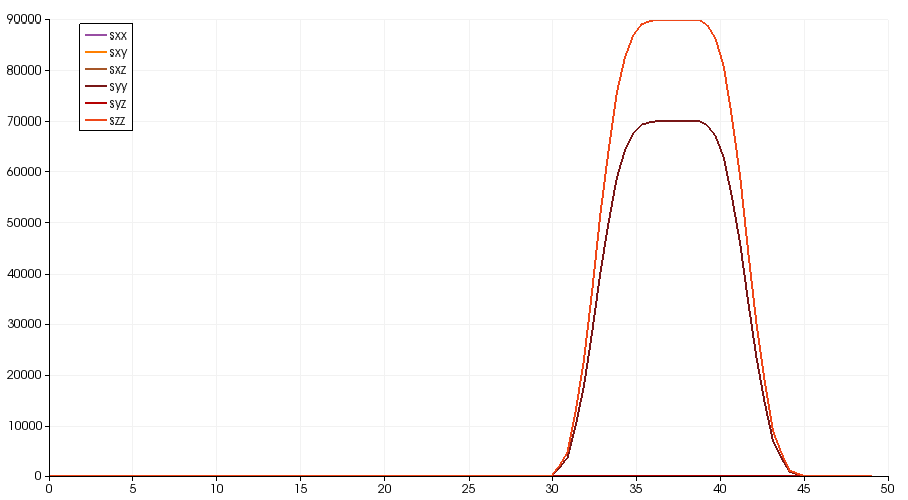
\includegraphics[width=0.8\textwidth]{png/p-wave-test/s/0005.png}
\caption{5-й временной слой}
\end{subfigure}
\begin{subfigure}[b]{0.5\textwidth}
\centering
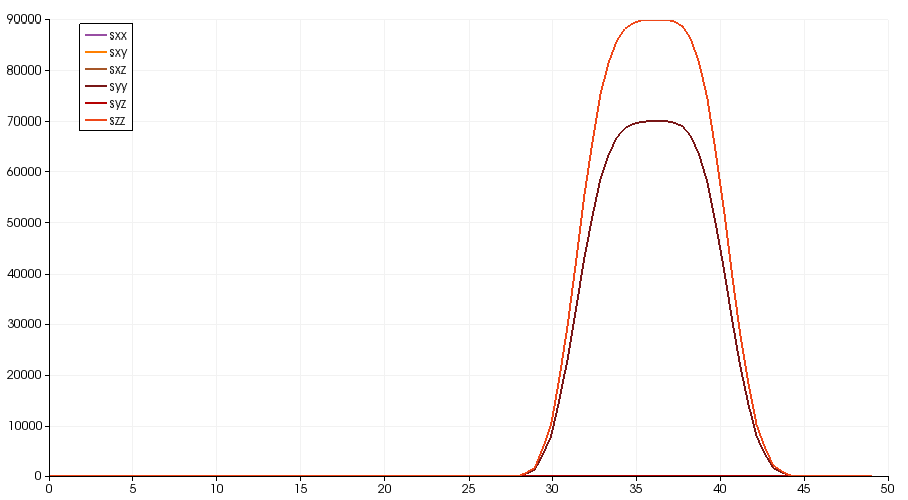
\includegraphics[width=0.8\textwidth]{png/p-wave-test/s/0007.png}
\caption{7-й временной слой}
\end{subfigure}
\begin{subfigure}[b]{0.5\textwidth}
\centering
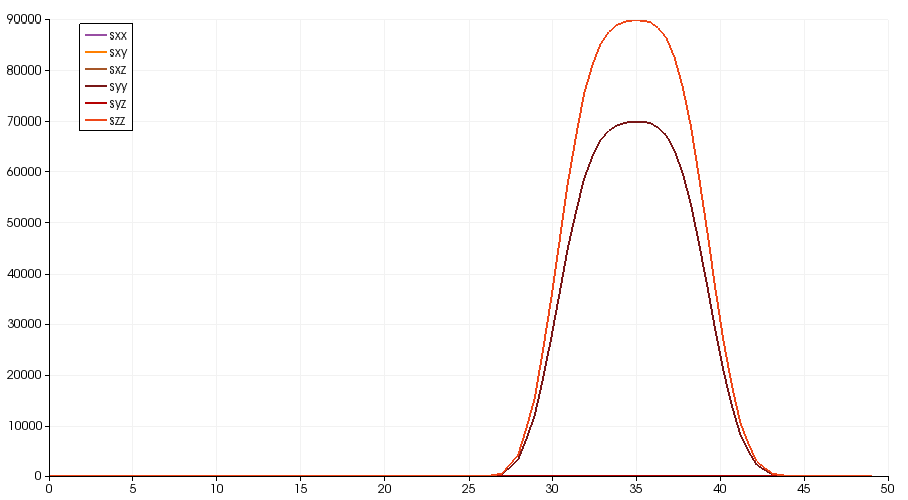
\includegraphics[width=0.8\textwidth]{png/p-wave-test/s/0009.png}
\caption{9-й временной слой}
\end{subfigure}
\begin{subfigure}[b]{0.5\textwidth}
\centering
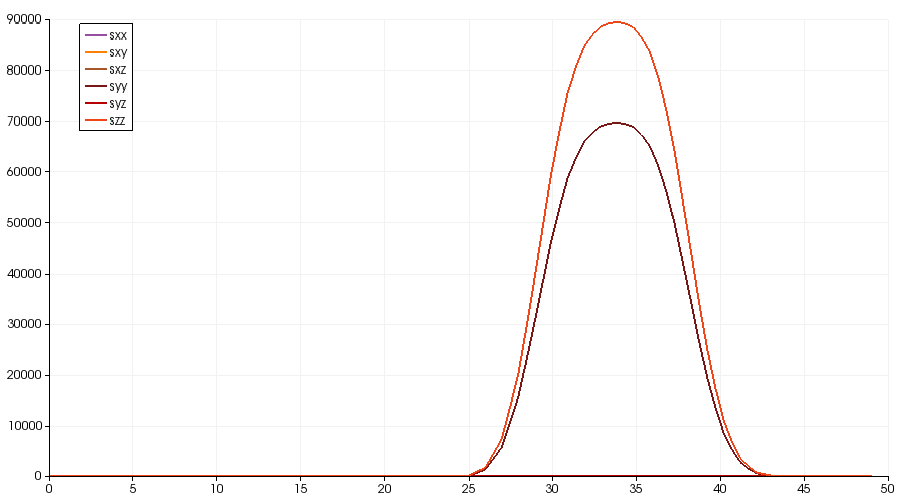
\includegraphics[width=0.8\textwidth]{png/p-wave-test/s/0011.png}
\caption{11-й временной слой}
\end{subfigure}
\begin{subfigure}[b]{0.5\textwidth}
\centering
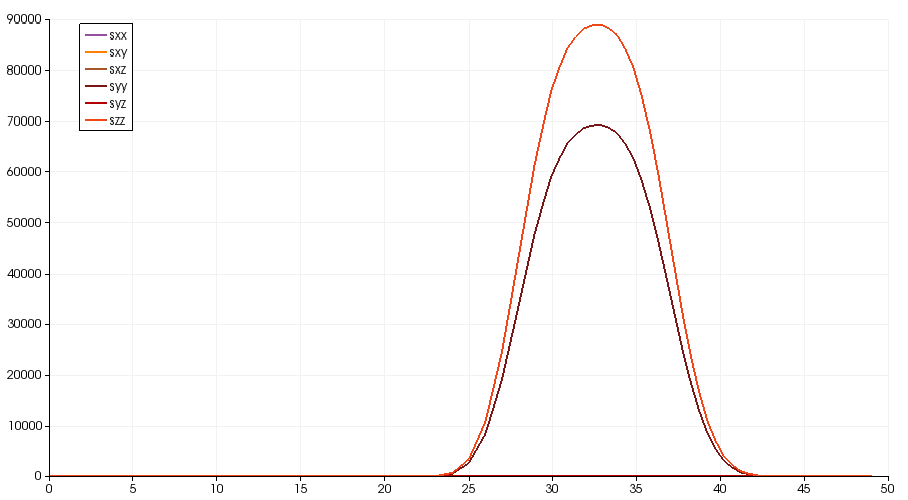
\includegraphics[width=0.8\textwidth]{png/p-wave-test/s/0013.png}
\caption{13-й временной слой}
\end{subfigure}
\begin{subfigure}[b]{0.5\textwidth}
\centering
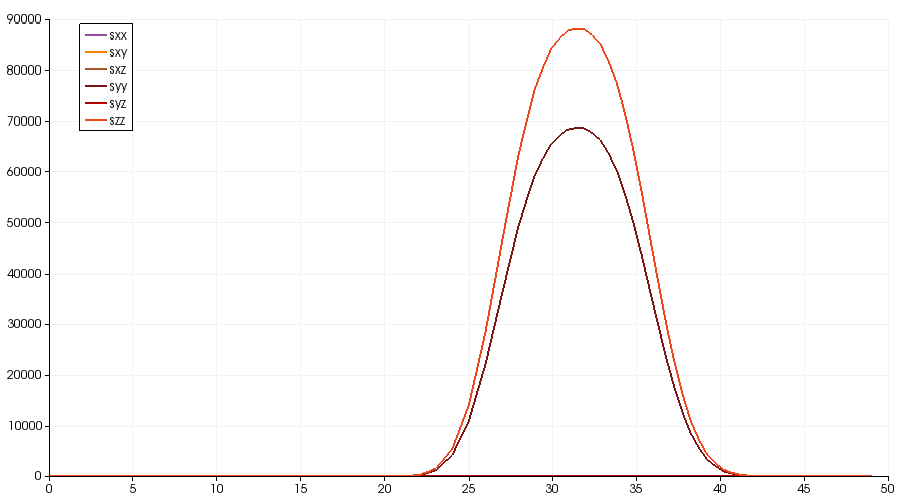
\includegraphics[width=0.8\textwidth]{png/p-wave-test/s/0015.png}
\caption{15-й временной слой}
\end{subfigure}
\caption{Распространение P-волны. Изображены компоненты тензора напряжений.}
\label{pic:p_wave}
\end{figure}


\subsubsection{Расчёт поперечной волны (S-волны)}
Пусть плоская S-волна в среде распространяется вдоль оси z. В этом случае аналитическое решение соответствующего одномерного уравнения дает следующие соотношения на параметры волны:
\begin{itemize}
\item $v_z=-f(z)\sqrt{\frac{\mu}{\rho}}=C_s$;
\item $v_x=v_y=0$;
\item $\sigma_{ij}=f(z)\mu$; для одной из пар $i \neq j$
\item $\sigma_{ij}=0$ для $i = j$.
\end{itemize}
Здесь $f(z)$ - произвольная функция, зависящая только от z и задающая форму волны.
Для расчёта распространения S-волны в кубе были использованы следующие безразмерные параметры: 
\begin{itemize}
\item $\lambda=70000$;
\item $\mu=10000$;
\item $\rho=1$.
\end{itemize}
На графиках (см. рис. \ref{pic:s_wave}) представлены результаты численного расчёта. Получено совпадение скорости волны с аналитическим решением:
\begin{itemize}
\item $v_z=C_s=100$.
\end{itemize}

\begin{figure}[htp]
\begin{subfigure}[b]{0.5\textwidth}
\centering
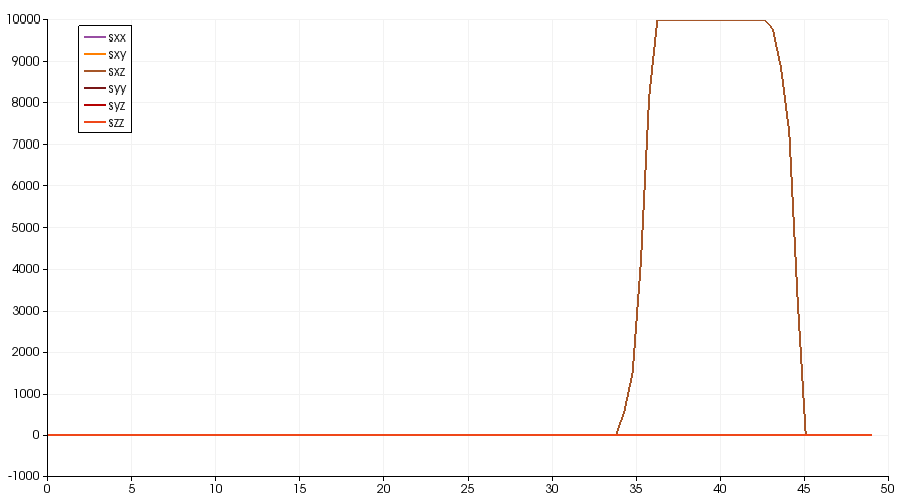
\includegraphics[width=0.8\textwidth]{png/s-wave-test/s/0001.png}
\caption{1-й временной слой.}
\end{subfigure}
\begin{subfigure}[b]{0.5\textwidth}
\centering
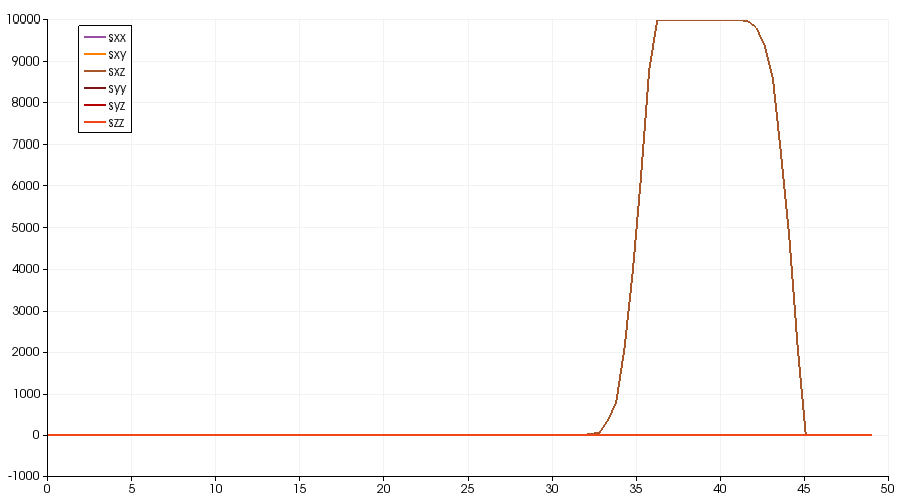
\includegraphics[width=0.8\textwidth]{png/s-wave-test/s/0003.png}
\caption{3-й временной слой.}
\end{subfigure}
\begin{subfigure}[b]{0.5\textwidth}
\centering
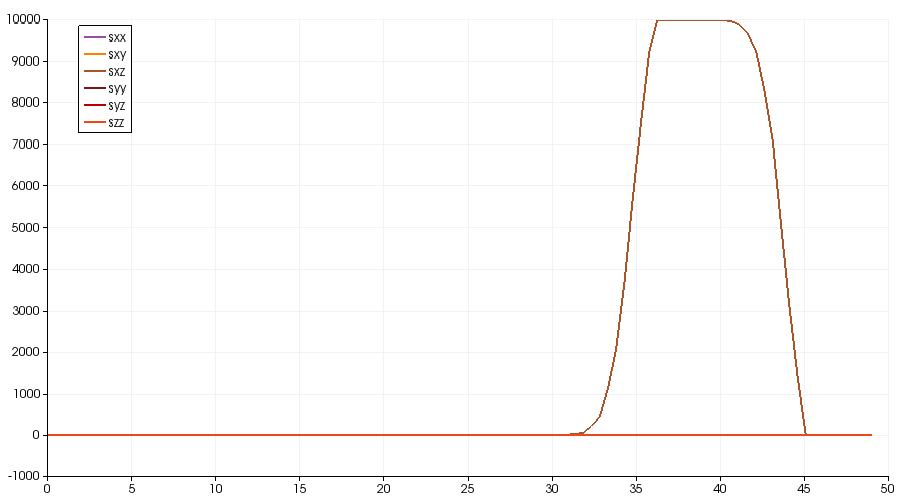
\includegraphics[width=0.8\textwidth]{png/s-wave-test/s/0005.png}
\caption{5-й временной слой.}
\end{subfigure}
\begin{subfigure}[b]{0.5\textwidth}
\centering
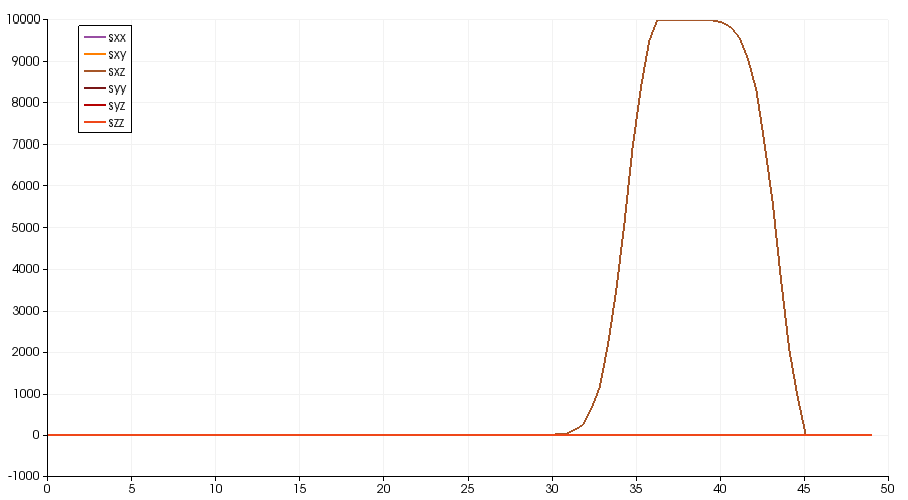
\includegraphics[width=0.8\textwidth]{png/s-wave-test/s/0007.png}
\caption{7-й временной слой.}
\end{subfigure}
\begin{subfigure}[b]{0.5\textwidth}
\centering
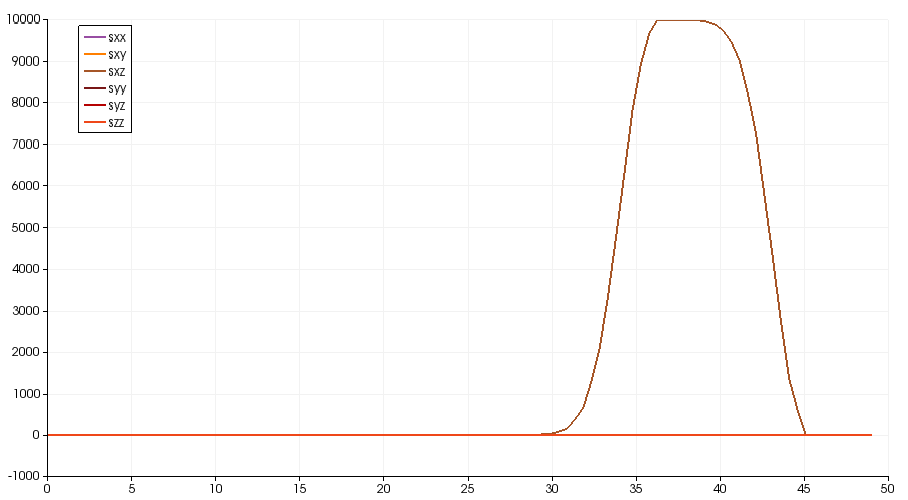
\includegraphics[width=0.8\textwidth]{png/s-wave-test/s/0009.png}
\caption{9-й временной слой.}
\end{subfigure}
\begin{subfigure}[b]{0.5\textwidth}
\centering
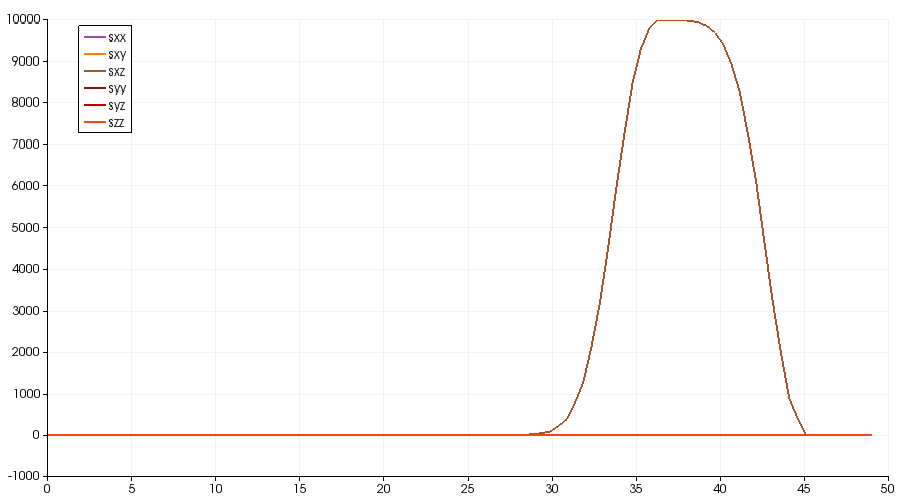
\includegraphics[width=0.8\textwidth]{png/s-wave-test/s/0011.png}
\caption{11-й временной слой.}
\end{subfigure}
\begin{subfigure}[b]{0.5\textwidth}
\centering
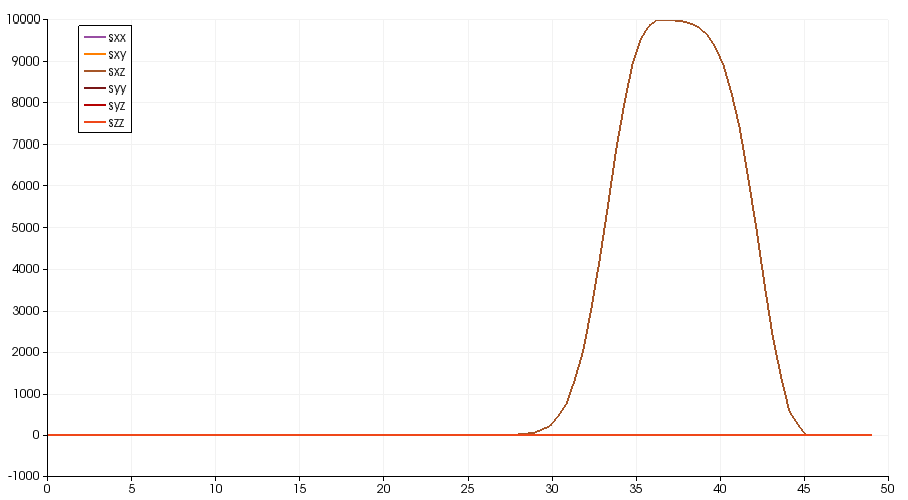
\includegraphics[width=0.8\textwidth]{png/s-wave-test/s/0013.png}
\caption{13-й временной слой.}
\end{subfigure}
\begin{subfigure}[b]{0.5\textwidth}
\centering
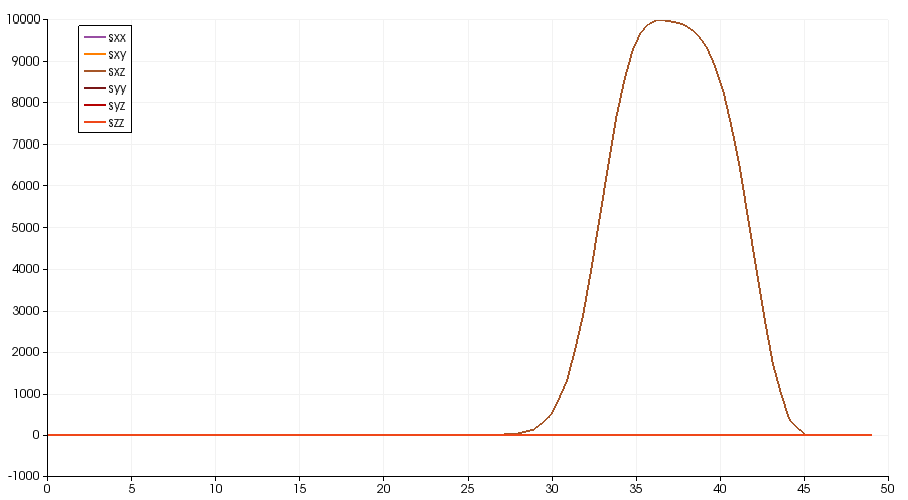
\includegraphics[width=0.8\textwidth]{png/s-wave-test/s/0015.png}
\caption{15-й временной слой.}
\end{subfigure}
\caption{Распространение S-волны. Изображены компоненты тензора напряжений.}
\label{pic:s_wave}
\end{figure}


\clearpage
\newpage


\subsection{Поверхностные волны}

\subsubsection{Отражение плоской волны от свободной границы}

При наличии в среде границ картина заметно усложняется. Однако для прямолинейного фронта и прямолинейно границы существует точное решение, а в остальных интересующих нас случаях можно, в некотором приближении, свести нелинейную границу и нелинейный фронт к наборам линейных участков.

Рассмотрим упругое полупространство с бесконечной плоской свободной границей. В отличие от среды, бесконечной во всех направлениях, мы можем наблюдать три вида волн: P-волны, SH-волны и SV-волны. P-волны – это продольные волны, в них частицы вещества движутся поступательно. SH- и SV-волны – поперечные, их фронт распространяется с одинаковой скоростью, перпендикулярной  скоростям частиц вещества. Разница между ними заключается в том, что мгновенная скорость частиц в SH-волне параллельна плоскости границы. Соответственно, в SV-волне она направлена под углом к границе. Заметим, что в двухмерной постановке задачи SH-волны наблюдать нельзя.

В однородной среде эти волны распространяются независимо, но при отражении от границы ситуация меняется. SH-волны распространяются и отражаются так же независимо, а P- и SV-волны генерируют друг друга при отражении. Приведем математические соотношения для падающих (P, SV) и отраженных волн.

\begin{figure}[h]
\center{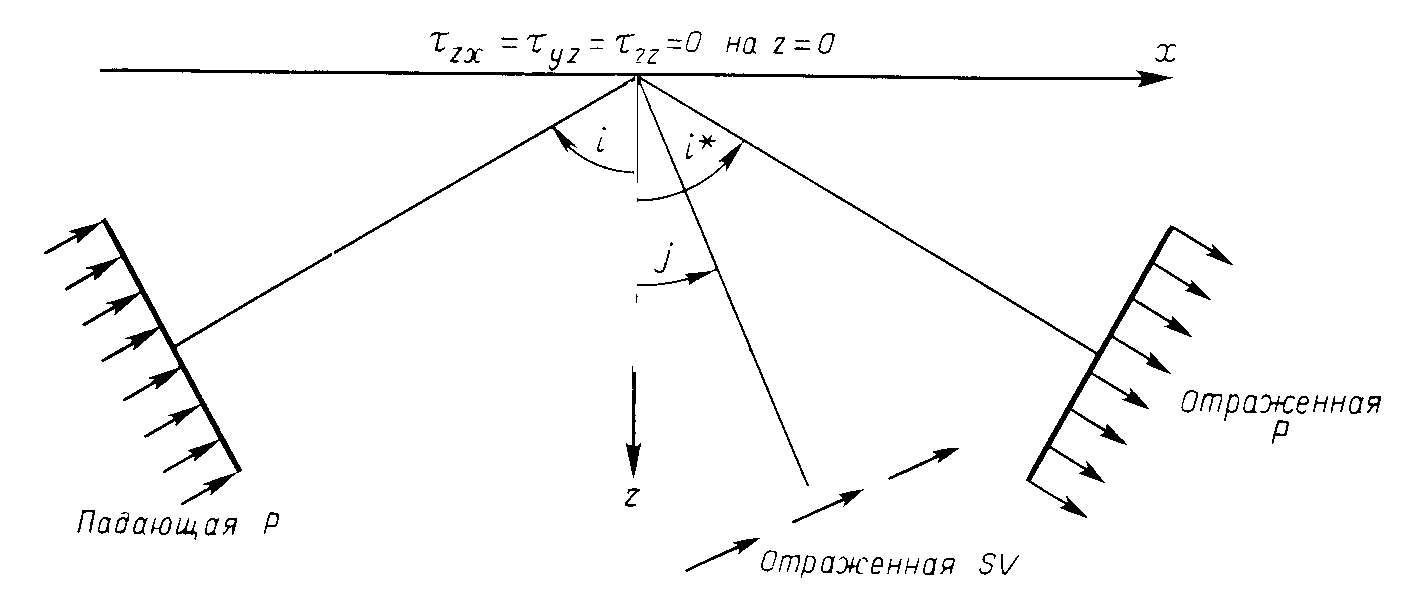
\includegraphics[width=\textwidth]{png/waves-analytics/reflection-scheme.png}}
\caption{Система лучей и координаты, используемые при изучении отраженных волн.}
\end{figure}

Из условие свободной границы мы получаем, что $i = i^*$ (углы падения и отражения Р-волны равны), $\frac{\sin{i}}{\alpha} = \frac{\sin{j}}{\beta} = p$. Здесь $p$ обозначает лучевой параметр, $\alpha$ – скорость продольной волны, $\beta$ – скорость поперечной волны. 

\begin{figure}[h]
\center{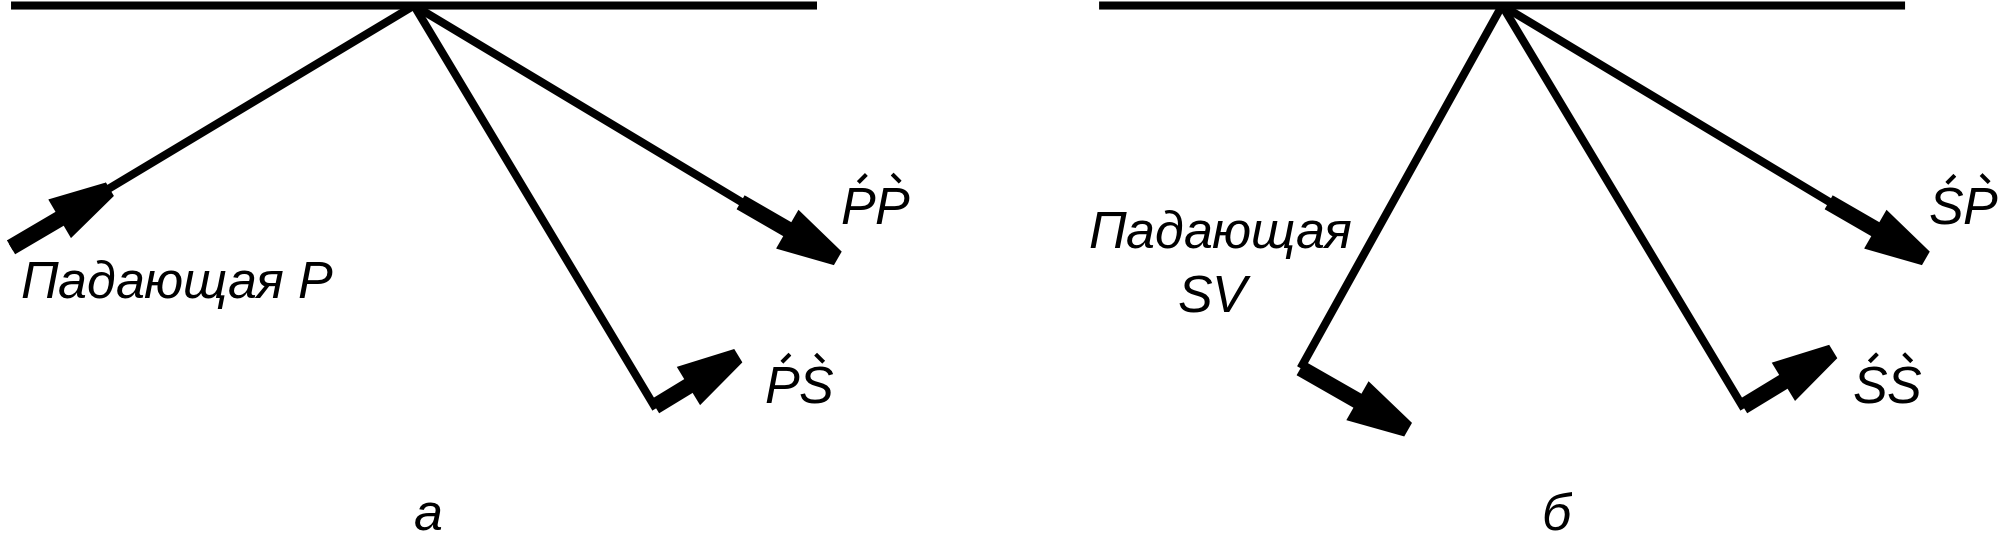
\includegraphics[width=\textwidth]{png/waves-analytics/reflection-p-sv.png}}
\caption{Обозначения и правило знаков для коэффициентов отражения плоских волн Р и SV от свободной поверхности.}
\end{figure}

Для указанных волн получаются следующие амплитудные соотношения для потенциалов:
\begin{eqnarray}
PP = \frac{ -(\frac{1}{\beta^2} - 2p^2)^2 + 4p^2\frac{\cos{i}}{\alpha}\frac{\cos{j}}{\beta} }{ (\frac{1}{\beta^2} - 2p^2)^2 + 4p^2\frac{\cos{i}}{\alpha}\frac{\cos{j}}{\beta} }, \\
PS = \frac{ 4\frac{\alpha}{\beta}p\frac{\cos{i}}{\alpha}(\frac{1}{\beta^2} - 2p^2)^2 }{ (\frac{1}{\beta^2} - 2p^2)^2 + 4p^2\frac{\cos{i}}{\alpha}\frac{\cos{j}}{\beta} }.
\end{eqnarray}

\begin{eqnarray}
SP = \frac{ 4\frac{\beta}{\alpha}p\frac{\cos{j}}{\beta}(\frac{1}{\beta^2} - 2p^2)^2 }{ (\frac{1}{\beta^2} - 2p^2)^2 + 4p^2\frac{\cos{i}}{\alpha}\frac{\cos{j}}{\beta} }, \\
SS = \frac{ (\frac{1}{\beta^2} - 2p^2)^2 - 4p^2\frac{\cos{i}}{\alpha}\frac{\cos{j}}{\beta} }{ (\frac{1}{\beta^2} - 2p^2)^2 + 4p^2\frac{\cos{i}}{\alpha}\frac{\cos{j}}{\beta} }.
\end{eqnarray}

Чтобы получить амплитудные отношения для смещений, нужно коэффициент $PS$ умножить на $\alpha/\beta$, $SP$ -- на $\beta/\alpha$, $PP$ и $SS$ -- на 1.

SH-волна отражается, сохраняя прямолинейность фронта, под углом, равным углу падения, с прежней амплитудой.


\subsubsection{Волны Рэлея}

Рассмотрим задачу о свободных колебаниях упругого двухмерного полупространства в вакууме в отсутствие объемных сил (ось $x_1$ направлена вдоль границы, $x_2$ -- вглубь среды). Попробуем найти решение уравнений (1.3) в виде
\begin{eqnarray}
\phi = Ae^{-\alpha x_2 + iq(x_1-ct)}, \alpha > 0, \\
\psi_3 = Be^{-\beta x_2 + iq(x_1-ct)}, \beta > 0, \psi_1 = \psi_2 = 0,
\end{eqnarray}

где $q$ -- заданная частота, $c$ -- фазовая скорость, при граничных условиях $x_2 = 0, \sigma_{22} = \sigma_{11} = 0$. Предполагаем, что на бесконечности стремится к нулю. После подстановки получаем:
\begin{eqnarray}
u_1 = (iq Ae^{-\alpha x_2} - \beta Be^{-\beta x_2}) e^{iq(x_1-ct)}, \\
u_2 = (-\alpha Ae^{-\alpha x_2} - iq Be^{-\beta x_2}) e^{iq(x_1-ct)}.
\end{eqnarray}

После применения закона Гука, получим выражения для компонентов тензора напряжений на границе:
\begin{eqnarray}
\sigma_{22} = \mu q^2 [ (2-\frac{c^2}{c_2^2})A + 2i\sqrt{1-\frac{c^2}{c_2^2}}B ] e^{iq(x_1-ct)}, \\
\sigma_{12} = \mu q^2 [ -2i\sqrt{1-\frac{c^2}{c_1^2}}A + (2-\frac{c^2}{c_2^2})B ] e^{iq(x_1-ct)}.
\end{eqnarray}

Чтобы удовлетворить граничным условиям, нужно положить
\begin{eqnarray}
(2-\frac{c^2}{c_2^2})A + 2i\sqrt{1-\frac{c^2}{c_2^2}}B = 0, \\
-2i\sqrt{1-\frac{c^2}{c_1^2}}A + (2-\frac{c^2}{c_2^2})B = 0.
\end{eqnarray}

Определитель линейной однородной системы относительно А и В должен быть равен нулю.
\begin{eqnarray}
R = (2-k)^2 - 4\sqrt{(1-k)(1-\gamma k)} = 0, \\
k = \frac{c^2}{c_2^2}, \\
\gamma = \frac{c_2^2}{c_1^2} < 1.
\end{eqnarray}

Это уравнение определяет фазовую скорость $c$. Она не зависит от частоты $q$, а зависит лишь от соотношения $\frac{c_2}{c_1}$. Можно показать, что при любом соотношении уравнение (2.3) имеет корень, причем меньший единицы.

Таким образом, при любом соотношении коэффициентов Ляме в полупространстве будет наблюдаться приповерхностная волна, распространяющаяся со скорость, меньшей, чем скорость поперечных волн. Любая фиксированная точка изучаемого тела или породы при этом будет двигаться по эллипсу. Поскольку переносимая ими энергия сконцентрирована у поверхности, ее рассеивание происходит медленнее, чем в объемных волнах. Поэтому волны данного типа можно наблюдать на значительном удалении от источника возмущения.


\subsubsection{Волны Лэмба}

Волнами Лэмба называют упругие возмущения, распространяющиеся в твердой пластинке (слое) со свободными границами, у которых есть смещение как в направлении распространении волны, так и перпендикулярно плоскости пластинки. Иногда их называют нормальными волнами в пластинке.

\begin{figure}[h]
\center{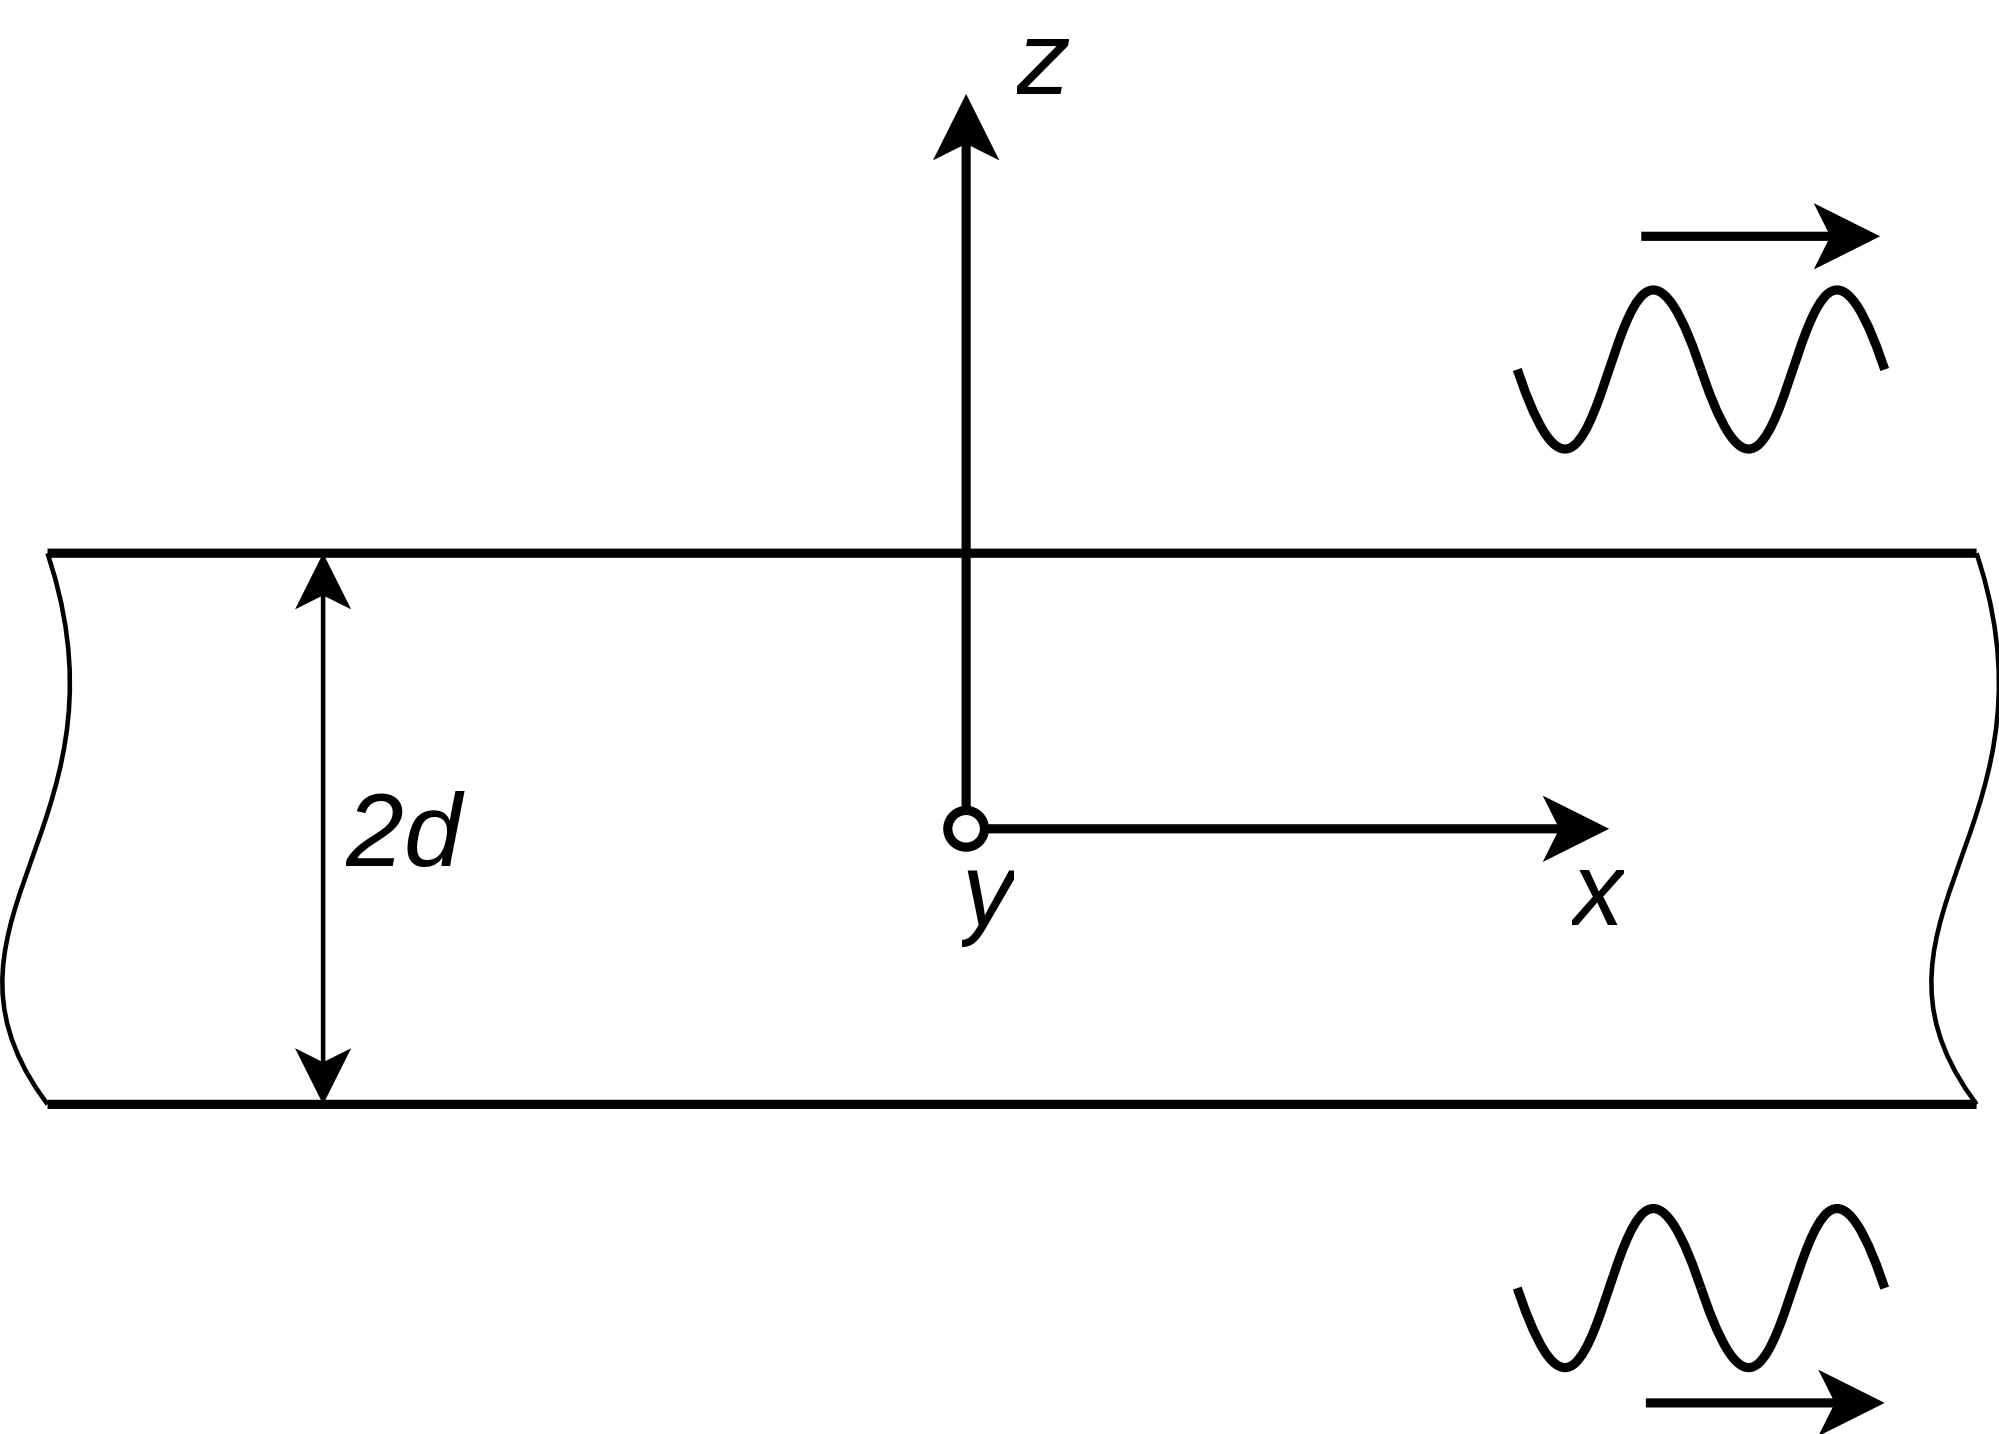
\includegraphics[width=0.5\textwidth]{png/waves-analytics/lamb-wave.png}}
\caption{Обозначения к задаче о распространении волн в пластинке.}
\end{figure}

Потенциалы, описывающие продольные и поперечные волны, имеют вид:
\begin{eqnarray}
U = \frac{\partial \phi}{\partial x} - \frac{\partial \psi}{\partial z}, \\
W = \frac{\partial \phi}{\partial z} + \frac{\partial \psi}{\partial x},
\end{eqnarray}

где $U$ и $W$ -- компоненты смещения. Запишем их в следующей форме:
\begin{eqnarray}
\phi = A_s \ch{qze^{ikx}} + B_a \sh{qze^{ikx}}, \\
\psi = D_s \sh{sze^{ikx}} + C_a \ch{sze^{ikx}}, \\
q = \sqrt{k^2 - k_l^2}, \\
s = \sqrt{k^2 - k_t^2}.
\end{eqnarray}

Здесь $As, Ba, Ds, Ca$ -- произвольные постоянные, $k$ -- волновое число Лэмба. Кроме того, компоненты тензора напряжения $\sigma_{xz}$ и $\sigma_{zz}$ должны обращаться в ноль на $z = \pm d$. Следовательно
\begin{eqnarray}
(k^2+s^2)\ch{qdA_s} + (k^2+s^2)\sh{qdB_a} + 2iks\sh{sdC_a} + 2iks\ch{sdD_s} = 0, \\
(k^2+s^2)\ch{qdA_s} - (k^2+s^2)\sh{qdB_a} - 2iks\sh{sdC_a} + 2iks\ch{sdD_s} = 0, \\
2ikq\sh{qdA_s} + 2ikq\ch{qdB_a} - (k^2+s^2)\ch{sdC_a} - (k^2+s^2)\sh{sdD_s} = 0, \\
-2ikq\sh{qdA_s} + 2ikq\ch{qdB_a} - (k^2+s^2)\ch{sdC_a} + (k^2+s^2)\sh{sdD_s} = 0.
\end{eqnarray}

Отсюда мы получаем два характеристических уравнения, которые определяют собственные значения волнового числа $k$.
\begin{eqnarray}
(k^2+s^2)^2\ch{qd}\sh{sd} - 4k^2qs\sh{qd}\ch{sd} = 0, \\
(k^2+s^2)^2\sh{qd}\ch{sd} - 4k^2qs\ch{qd}\sh{sd} = 0.
\end{eqnarray}

Следовательно, для искомых потенциалов:
\begin{eqnarray}
\phi = A_s\ch{q_{s}ze^{ik_{s}x}} + B_a\sh{q_{a}ze^{ik_{a}x}}, \\
\psi = \frac{ 2ik_{s}q_{s}\sh{q_{s}d} }{ (k_s^2+s_s^2)\sh{s_{s}d} } A_s\sh{s_{s}ze^{ik_{s}x}} + \frac{ 2ik_{a}q_{a}\sh{q_{a}d} }{ (k_a^2+s_a^2)\sh{s_{a}d} } B_a\ch{s_{a}ze^{ik_{a}x}}.
\end{eqnarray}

В результате получаем
\begin{eqnarray}
U = U_s + U_a, \\
W = W_s + W_a, \\
U_s = A k_s( \frac{\ch{q_s z}}{\sh{q_s d}} - \frac{2 q_s s_s}{k_s^2+s_s^2} \frac{\ch{s_s z}}{\sh{s_s d}} ) e^{i(k_s x - \omega t - \pi/2)}, \\
W_s = - A q_s( \frac{\sh{q_s z}}{\sh{q_s d}} - \frac{2 k_s^2}{k_s^2+s_s^2} \frac{\sh{s_s z}}{\sh{s_s d}} ) e^{i(k_s x - \omega t)}, \\
U_a = B k_a( \frac{\sh{q_a z}}{\ch{q_a d}} - \frac{2 q_a s_a}{k_a^2+s_a^2} \frac{\sh{s_a z}}{\ch{s_a d}} ) e^{i(k_a x - \omega t - \pi/2)}, \\
W_a = - B q_a( \frac{\ch{q_a z}}{\ch{q_a d}} - \frac{2 k_a^2}{k_a^2+s_a^2} \frac{\ch{s_a z}}{\ch{s_a d}} ) e^{i(k_a x - \omega t)}.
\end{eqnarray}

\begin{figure}[h]
\center{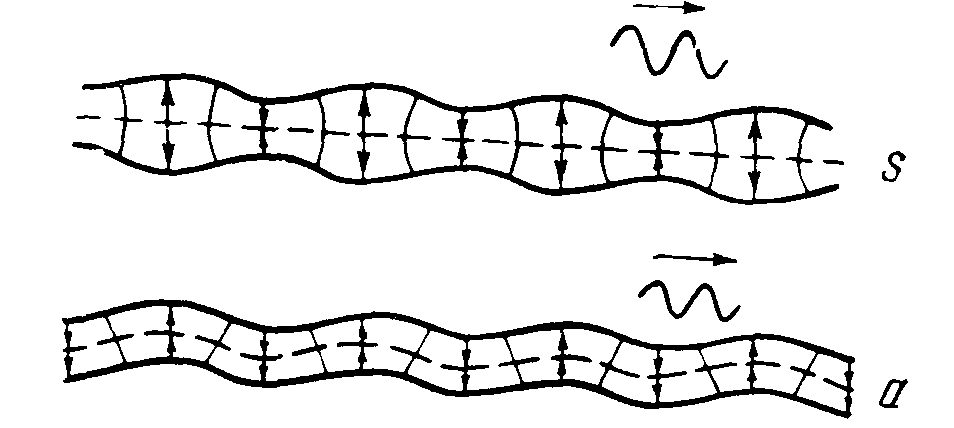
\includegraphics[width=0.5\textwidth]{png/waves-analytics/lamb-sym-ansym.png}}
\caption{Симметричные и антисимметричные волны.}
\end{figure}

Легко заметить, что полученные выражения описывают две группы волн, каждая из которых удовлетворяет волновым уравнениям движения и граничным условиям, т.е. может распространяться в пластинке независимо от другой. Первая группа волн (индекс $s$) описывает волны, в которых движение происходит симметрично плоскости $z = 0$. Соответственно, вторая – антисимметричные. 

В пластинке толщиной $2d$ может существовать определенное количество симметричных и антисимметричных волн Лэмба, отличающихся фазовыми и групповыми скоростями. Это количество определяется числом вещественных корней уравнений 2.6 и 2.7 соответственно. Каждый корень определяет волновое число и фазовую скорость соответствующей волны. Мнимые корни соответствуют экспоненциально затухающим движениям пластинки.

Заметим, что при увеличении пластинки свойства волн $s_0$ и $a_0$ (нулевые волны) меняются: они становятся все более «похожи» одна на другую. При стремлении толщины пластинки к бесконечности их фазовые скорости стремятся к фазовой скорости рэлеевской волны. Смещения становятся локализованными вблизи свободных границ пластинки. При интерференции вблизи от излучателя, где разность фаз между ними близка к нулю, их суммарное акустическое поле подобно акустическому полю рэлеевской волны, поэтому такую совокупность волн $s_0$ и $a_0$ можно назвать квазирэлеевской волной. По мере удаления от излучателя разность фаз между этими компонентами растет, и достигает на некотором расстоянии $L$ величины $\pi$. 
\begin{equation}
L = (\frac{1}{4} + \frac{1}{8(1- \eta_{R}^{2})} + \frac{1}{8(1- \eta_{R}^{2} \xi^2)} + \frac{1}{2- \eta_{R}^{2}} ) e^{2kR^d\sqrt{1- \eta_{R}^{2}}}
\end{equation}

На этом расстоянии квазирэлеевская волна, локализованная первоначально около той поверхности слоя, где расположен излучатель, «переходит» на противоположную поверхность. На расстоянии $2L$ происходит обратный «переход». Величина $L$ возрастает с увеличением толщины слоя, стремясь к бесконечности при стремлении толщины $d$ к бесконечности. То есть квазирэлеевская волна превращается в рэлеевскую.


\subsubsection{Отражение сферической волны от свободной границы}

Предположим, что однородное изотропное упругое тело со скоростями объемных волн $\alpha$ и $\beta$ и плотностью $\rho$ занимает полупространство $z > 0$.  В точке $z = h, x = 0, y = 0$ расположен точечный источник P-волн. Исследуем задачу о волнах P- и SV-, упрощенную осевой симметрией относительно вертикальной прямой, проходящей через источник. 

\begin{figure}[h]
\center{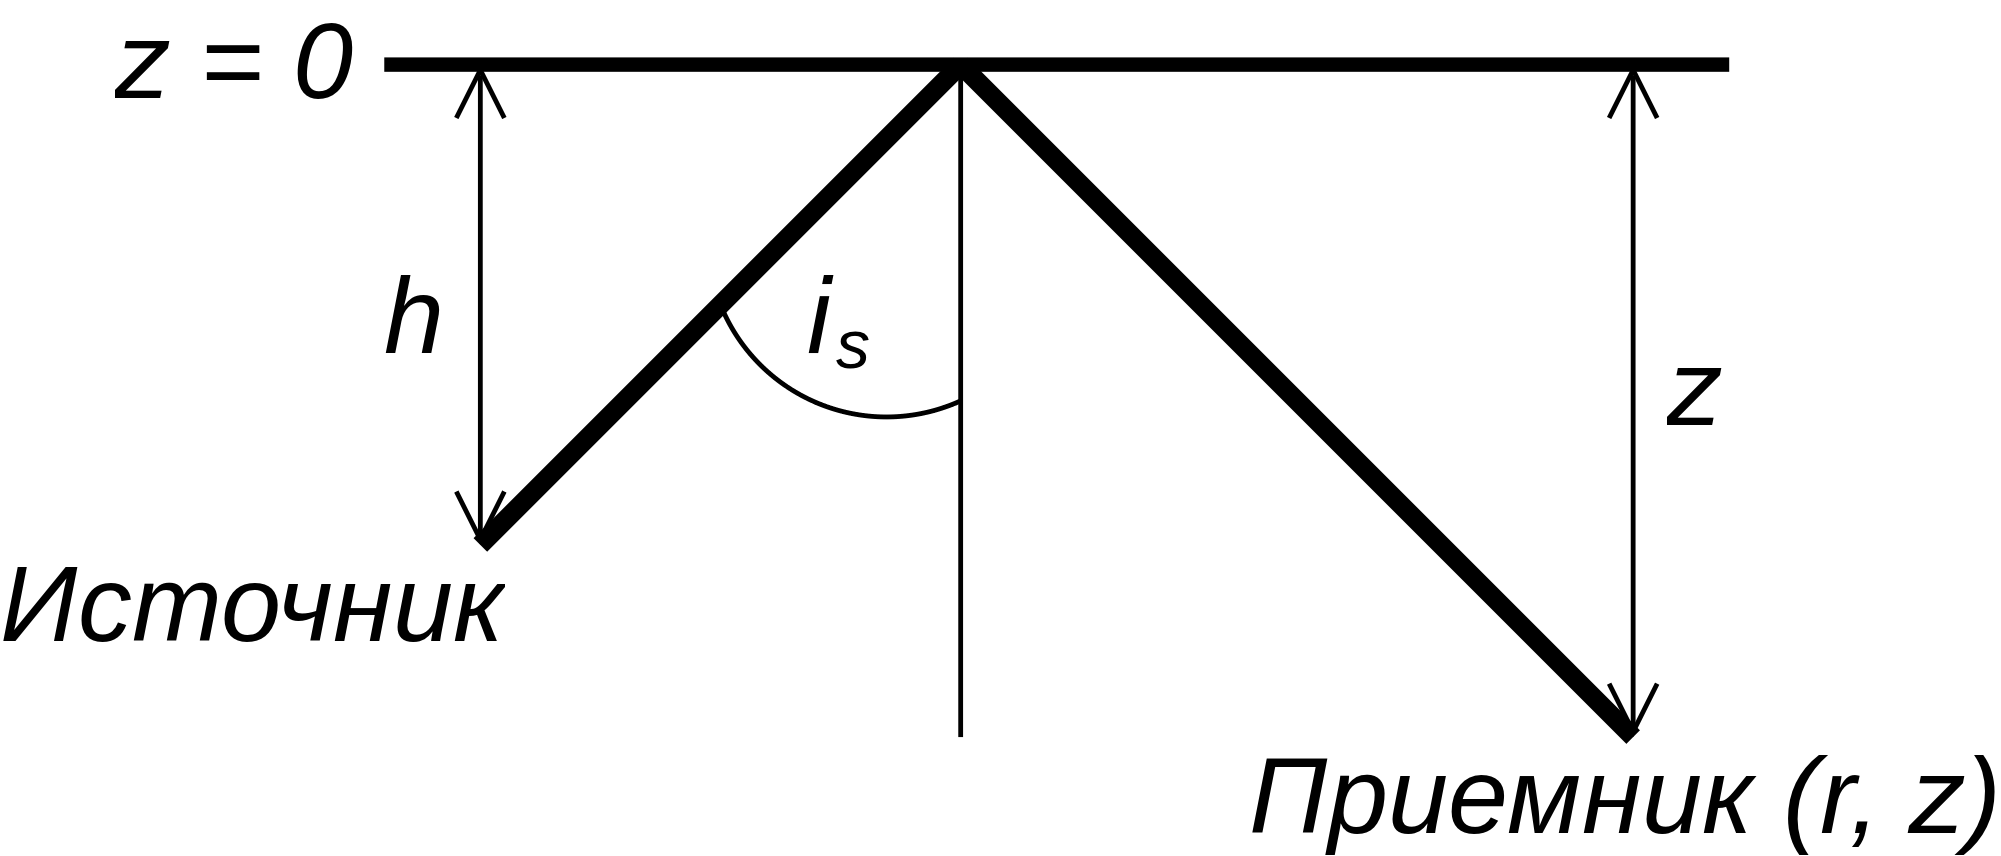
\includegraphics[width=0.5\textwidth]{png/waves-analytics/sphere-wave-reflection.png}}
\caption{Геометрия и обозначения к задаче об отражении сферической волны от свободной поверхности.}
\end{figure}

Тогда вектор смещения
\begin{equation}
\vec{u} = \nabla \phi + \nabla \times \nabla \times (0, 0, \psi)^T,
\end{equation}

а потенциалы удовлетворяют условиям
\begin{eqnarray}
\frac{\partial^2 \phi}{\partial t^2} = \frac{\Phi}{\rho} + \alpha^2 \nabla^2 \phi, \\
\frac{\partial^2 \psi}{\partial t^2} = \frac{\Psi}{\rho} + \beta^2 \nabla^2 \psi,
\end{eqnarray}

где $\Phi$ и $\Psi$ -- потенциалы объёмной силы:
\begin{equation}
\vec{f} = \rho \frac{\partial^2 \vec{u}}{\partial t^2} - (\lambda + 2\mu)\nabla(\nabla\vec{u}) + \mu \nabla \times (\nabla \times \vec{u} ) = \nabla \Phi + \nabla \times \nabla \times (0, 0, \psi)^T.
\end{equation}

Источник генерирует только P-волну:
\begin{eqnarray}
\Phi = A 4\pi \rho \alpha^2 \delta(x)\delta(y)\delta(z-h)e^(-i \omega t),
\Psi = 0,
\end{eqnarray}

то есть
\begin{equation}
\phi^*(\vec{x}, t) = A \frac{1}{R} exp[i\omega (\frac{R}{\alpha} - t)],
\end{equation}

где $\phi^*(\vec{x}, t)$ -- падающая волна, $R = (x^2 + y^2 + (z-h)^2)^{1/2}$.

Сумма падающей и отражённой P-волны:
\begin{equation}
\phi = A i \omega exp(-i \omega t) \int_0^\infty { \frac{p}{\xi}J_0(\omega pr)exp(i \omega \xi |z - h|) \mathrm{d}p}
	+ A i \omega exp(-i \omega t) \int_0^\infty { PP \frac{p}{\xi}J_0(\omega pr)exp(i \omega \xi (z + h)) \mathrm{d}p}.
\end{equation}

Отраженная SV-волна:
\begin{equation}
\phi = A i \omega exp(-i \omega t) \int_0^\infty { (\frac{1}{i \omega p} \frac{\beta}{\alpha} PS) \frac{p}{\xi}J_0(\omega pr)exp(i \omega \xi |\xi h + \eta z|) \mathrm{d}p}.
\end{equation}

Обобщенное отражение P-волны распадается, с увеличением расстояния, на три различных типа P-волн: отраженная P-волна, поверхностная S-волна и P-компонента рэлеевской волны. Из тех же уравнений мы можем получить оценку расстояния формирования волны Рэлея:
\begin{equation}
\tg{i_s} = \frac{r}{z+h} < \frac{C_R}{(\alpha^2 - C_R^2)^{1/2}}.
\end{equation}

Аналогично, на три типа распадается отраженная SV-волна. 


\subsubsection{Расчёт отражения сферической волны}
Для проверки изотропии схемы и корректности расчёта при отражении от границ был произведён расчёт модельной задачи об отражении сферической волны от свободной поверхности. Параметры расчёта:
\begin{itemize}
\item $\lambda=20000$;
\item $\mu=10000$;
\item $\rho=1$.
\end{itemize}
На рис. \ref{pic:sphere_wave_reflection_2d} изображены результаты расчётов. Видны три группы волн -- исходная волна, распространяющаяся вглубь полупространства, отражённая продольная волна со сферическим фронтом, отражённая поперечная волна со сферическим фронтом и «окном» на нормали к поверхности.

\begin{figure}[h]
\center{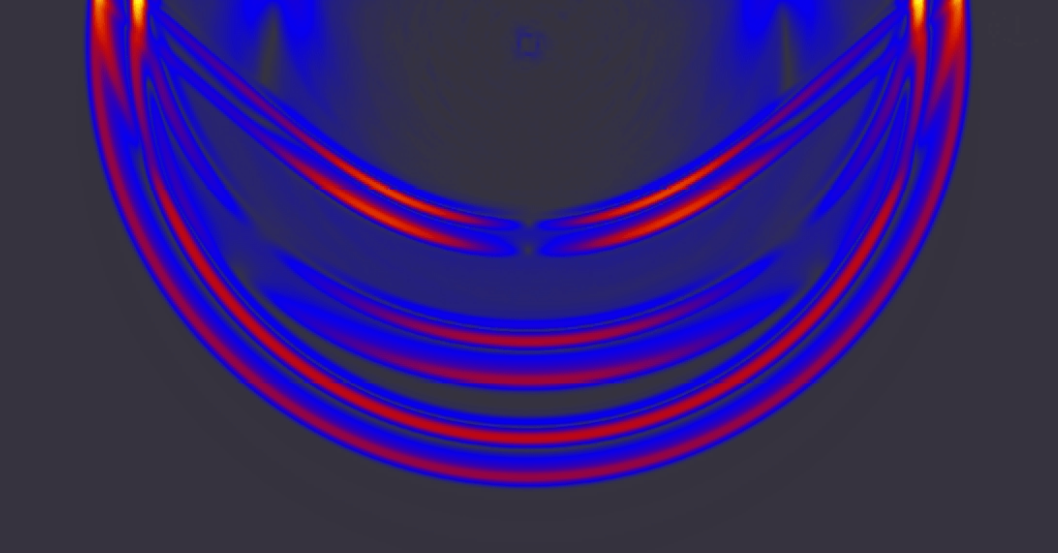
\includegraphics[width=\textwidth]{png/2d/sphere-explosion-02.png}}
\caption{Отражение сферической волны от свободной границы.}
\label{pic:sphere_wave_reflection_2d}
\end{figure}


\subsubsection{Расчёт волны Лэмба}

\todo{Описать постановку}

\begin{figure}[htp]
\begin{subfigure}[b]{\textwidth}
\centering
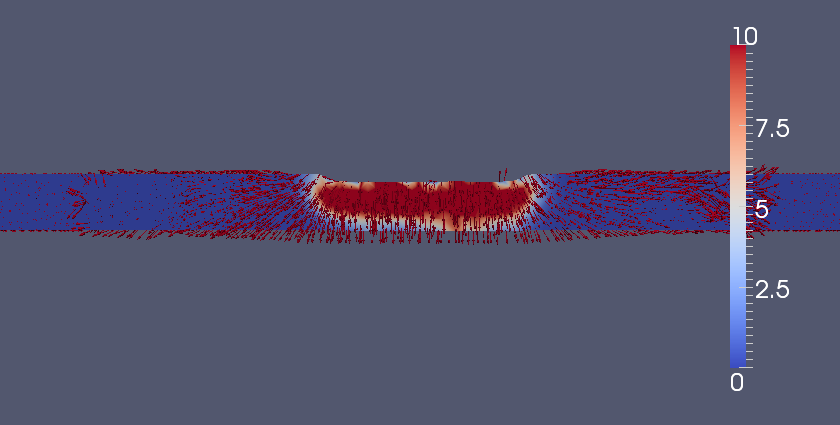
\includegraphics[width=0.6\textwidth]{png/lamb-wave/010.png}
\caption{10-й временной слой}
\end{subfigure}
\begin{subfigure}[b]{\textwidth}
\centering
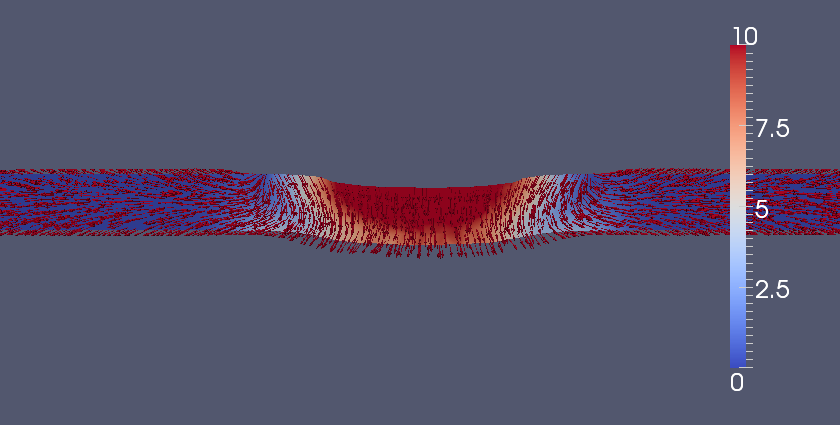
\includegraphics[width=0.6\textwidth]{png/lamb-wave/050.png}
\caption{50-й временной слой}
\end{subfigure}
\begin{subfigure}[b]{\textwidth}
\centering
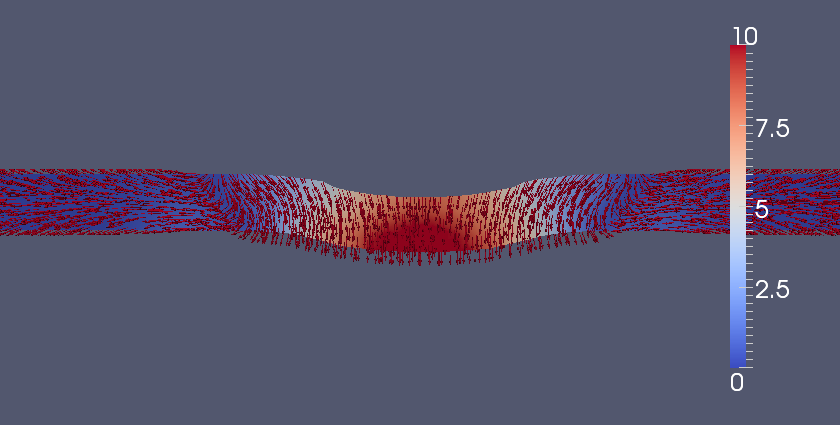
\includegraphics[width=0.6\textwidth]{png/lamb-wave/090.png}
\caption{90-й временной слой}
\end{subfigure}
\begin{subfigure}[b]{\textwidth}
\centering
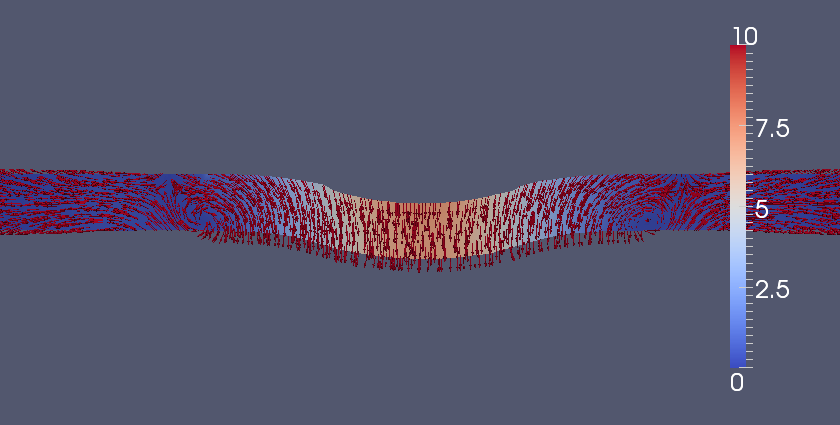
\includegraphics[width=0.6\textwidth]{png/lamb-wave/130.png}
\caption{130-й временной слой}
\end{subfigure}
\caption{Формирование волны Лэмба. Цветом показан модуль скорости.}
\label{pic:lamb_wave}
\end{figure}


\clearpage
\newpage


\subsection{Волны на контактной границе}

\subsubsection{Преломление на плоской контактной границе}

Аналогично случаю со свободной границей, рассмотрим прохождение плоского волнового фронта через плоский контакт между двумя бесконечными средами. Условие на контакте считается полным слипанием: все компоненты скорости и напряжений равны. В случае контакта мы также рассматриваем P-, SV- и SH-волны. SH-волны распространяются, преломляются и отражаются так же независимо, а P- и SV-волны так же генерируют друг друга при отражении и преломлении. 

Приведем математические соотношения для падающих, преломленных и отраженных SH-волн. Обозначения приведены на рисунке 3.1.

\begin{figure}[h]
\center{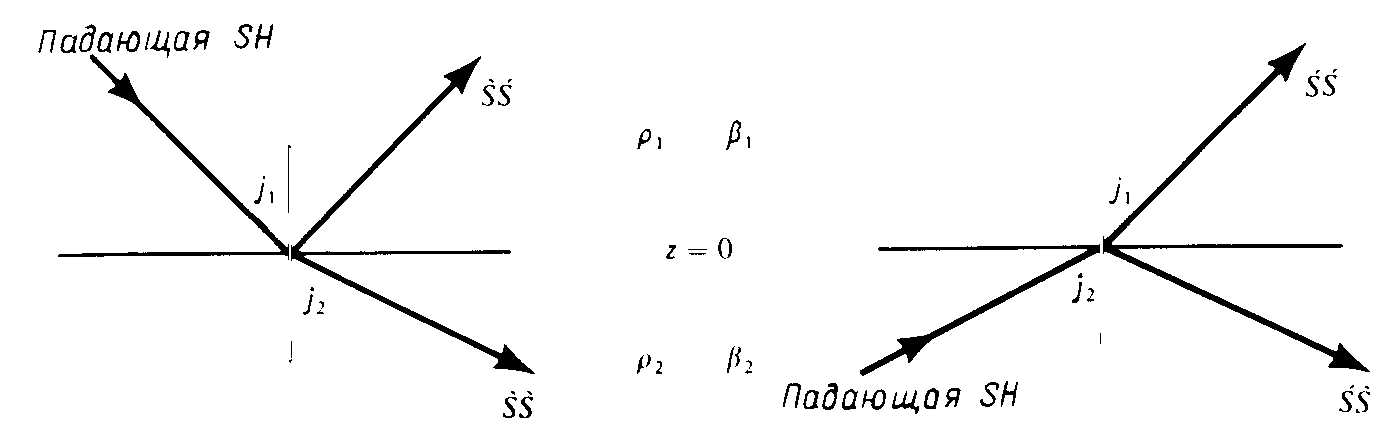
\includegraphics[width=\textwidth]{png/waves-analytics/contact-1.png}}
\caption{Обозначения для четырех возможных коэффициентов отражения и преломления для задачи о падении волн SH.}
\end{figure}

Исходя из непрерывности y-компоненты смещения и yz-компоненты напряжения мы находим коэффициенты рассеяния:
\begin{eqnarray}
SS = \frac{\rho_1 \beta_1 \cos{j_1} - \rho_2 \beta_2 \cos{j_2}}{\Delta}, \\
SS = \frac{2 \rho_2 \beta_2 \cos{j_2}}{\Delta}, \\
SS = \frac{2 \rho_1 \beta_1 \cos{j_1}}{\Delta}, \\
SS = - SS, \\
\Delta = \rho_1 \beta_1 \cos{j_1} + \rho_2 \beta_2 \cos{j_2}.
\end{eqnarray}

Приведем математические соотношения для падающих, преломленных и отраженных P- и SV-волн. Обозначения приведены на рисунке 3.2.

\begin{figure}[h]
\center{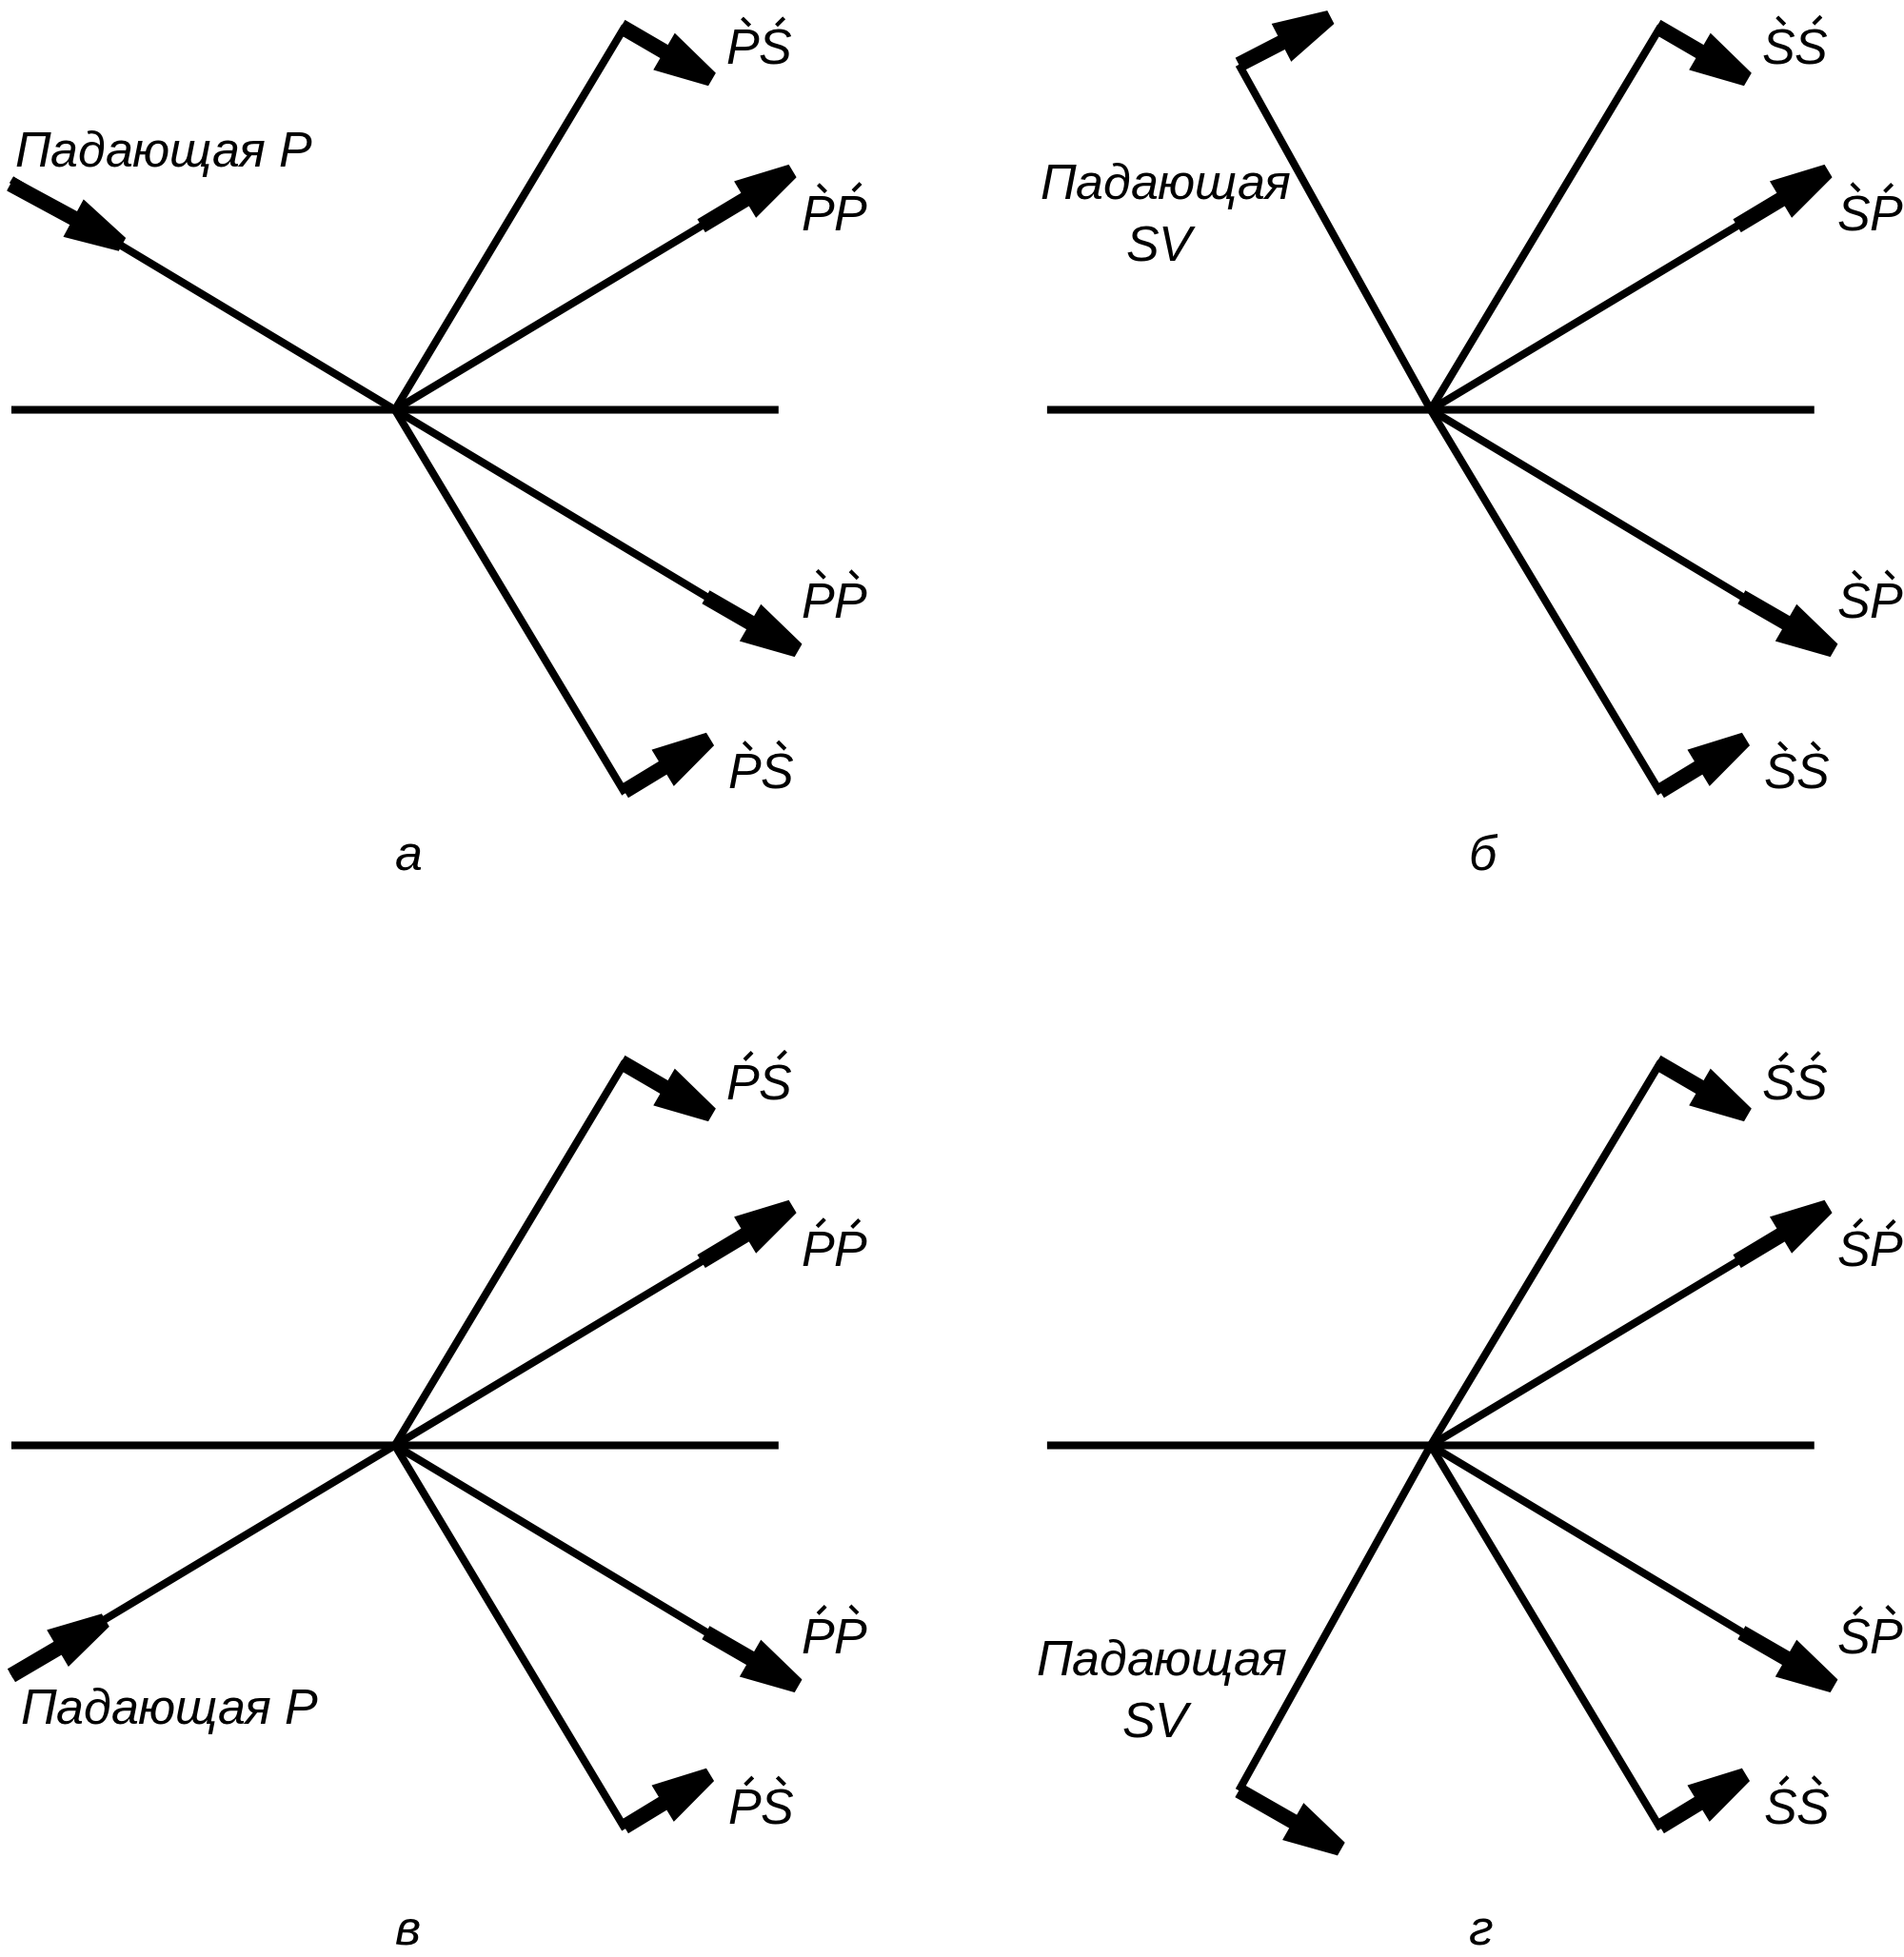
\includegraphics[width=\textwidth]{png/waves-analytics/contact-2.png}}
\caption{Обозначения для 16 возможных коэффициентов отражения и преломления, возникающих в задачах о волнах P- и SV- на жесткой границе между двумя различными твердыми полупространствами.}
\end{figure}

Коэффициенты рассеяния удобно представить в виде матрицы:
\begin{displaymath}
\left( \begin{array}{cccc}
PP & SP & PP & SP \\
PS & SS & PS & SS \\
PP & SP & PP & SP \\
PS & SS & PS & SS \\
\end{array} \right)
\end{displaymath} 

где каждый столбец представляет собой четыре волны, рассеянные на границе, на которую падает волна определенного типа. Из непрерывности $u_x, u_y, \tau_{zx}, \tau_{zz}$ получаем четыре уравнения с четырьмя неизвестными:
\begin{eqnarray}
\sin{i_1(P_1 + P_1)} + \cos{j_1(S_1 + S_1)} = \sin{i_2(P_2 + P_2)} + \cos{j_2(S_2 + S_2)}, \\
\cos{i_1(P_1 - P_1)} - \sin{j_1(S_1 - S_1)} = \cos{i_2(P_2 - P_2)} - \sin{j_2(S_2 s S_2)}, \\
2 \rho_1 \beta_1^2 p \cos{i_1(P_1 - P_1)} + \rho_1 \beta_1 (1 - 2 \beta_1^2 p^2) (S_1 - S_1) = 2 \rho_2 \beta_2^2 p \cos{i_2(P_2 - P_2)} + \rho_2 \beta_2 (1 - 2 \beta_2^2 p^2) (S_2 - S_2), \\
\rho_1 \alpha_1 (1 - 2 \beta_1^2 p^2) (P_1 + P_1) - 2 \rho_1 \beta_1^2 p \cos{j_1(S_1 + S_1)} = \rho_2 \alpha_2 (1 - 2 \beta_2^2 p^2) (P_2 + P_2) - 2 \rho_2 \beta_2^2 p \cos{j_2(S_2 + S_2)}.
\end{eqnarray}

В результате получаем коэффициенты матрицы рассеяния:
\begin{eqnarray}
PP = [ ( b\frac{\cos{i_1}}{\alpha_1} - c\frac{\cos{i_2}}{\alpha_2} )F - ( a + d\frac{\cos{i_1}}{\alpha_1}\frac{\cos{j_2}}{\beta_2} )Hp^2 ] / D, \\
PS = -2 \frac{\cos{i_1}}{\alpha_1} (ab + cd \frac{\cos{i_2}}{\alpha_2} \frac{\cos{j_2}}{\beta_2} ) p \alpha_1 / (\beta_1 D), \\
PP = 2 \rho_1 \frac{\cos{i_1}}{\alpha_1} F \alpha_1 / (\alpha_2 D), \\
PS = 2 \rho_1 \frac{\cos{i_1}}{\alpha_1} H p \alpha_1 / (\beta_2 D), \\
SP = -2 \frac{\cos{i_1}}{\beta_1} (ab + cd \frac{\cos{i_2}}{\alpha_2} \frac{\cos{j_2}}{\beta_2} ) p \beta_1 / (\alpha_1 D), \\
SS = - [ ( b\frac{\cos{j_1}}{\beta_1} - c\frac{\cos{j_2}}{\beta_2} )E - ( a + d\frac{\cos{i_2}}{\alpha_2}\frac{\cos{j_1}}{\beta_1} )Gp^2 ] / D, \\
SP = - 2 \rho_1 \frac{\cos{j_1}}{\beta_1} Gp \beta_1 / (\alpha_2 D), \\
SS = 2 \rho_1 \frac{\cos{j_1}}{\beta_1} E \beta_1 / (\beta_2 D), \\
PP = 2 \rho_2 \frac{\cos{i_2}}{\alpha_2} F \alpha_2 / (\alpha_1 D), \\
PS = - 2 \rho_2 \frac{\cos{i_2}}{\alpha_2} Gp \alpha_2 / (\beta_1 D), \\
PP = - [ ( b\frac{\cos{i_1}}{\alpha_1} - c\frac{\cos{i_2}}{\alpha_2} )F + ( a + d\frac{\cos{i_2}}{\alpha_2}\frac{\cos{j_1}}{\beta_1} )Gp^2 ] / D, \\
PS = 2 \frac{\cos{i_2}}{\alpha_2} (ac + bd \frac{\cos{i_1}}{\alpha_1} \frac{\cos{j_1}}{\beta_1} ) p \alpha_2 / (\beta_2 D), \\
SP = 2 \rho_2 \frac{\cos{j_2}}{\beta_2} Hp \beta_2 / (\alpha_1 D), \\
SS = 2 \rho_2 \frac{\cos{j_2}}{\beta_2} E \beta_2 / (\beta_1 D), \\
SP = 2 \frac{\cos{j_2}}{\beta_2} (ac + bd \frac{\cos{i_1}}{\alpha_1} \frac{\cos{j_1}}{\beta_1} ) p \beta_2 / (\alpha_2 D), \\
SS = [ ( b\frac{\cos{j_1}}{\beta_1} - c\frac{\cos{j_2}}{\beta_2} )E + ( a + d\frac{\cos{i_1}}{\alpha_1}\frac{\cos{j_2}}{\beta_2} )Hp^2 ] / D,
\end{eqnarray}

где
\begin{eqnarray}
E = b \frac{\cos{i_1}}{\alpha_1} + c \frac{\cos{i_2}}{\alpha_2}, \\
F = b \frac{\cos{j_1}}{\beta_1} + c \frac{\cos{j_2}}{\beta_2}, \\
G = a - d \frac{\cos{i_1}}{\alpha_1} \frac{\cos{j_2}}{\beta_2}, \\
H = a - d \frac{\cos{i_2}}{\alpha_2} \frac{\cos{j_1}}{\beta_1}, \\
D = EF + GHp^2 = \det{M}(\alpha_1 \alpha_2 \beta_1 \beta_2), \\
a = \rho_2 (1 - 2 \beta_2^2 p^2) - \rho_1 (1 - 2 \beta_1^2 p^2), \\
b = \rho_2 (1 - 2 \beta_2^2 p^2) + 2 \rho_1 \beta_1^2 p^2, \\
c = \rho_1 (1 - 2 \beta_1^2 p^2) + 2 \rho_2 \beta_2^2 p^2, \\
d = 2 (\rho_2 \beta_2^2 + \rho_1 \beta_1^2).
\end{eqnarray}


\subsubsection{Волны Стоунли}

При определенном соотношении параметров материалов сред по аналогии с волнами Рэлея возникают волны Стоунли. Например, такие волны могут всегда существовать на границе твердого тела и жидкости. Так же, как и волны Рэлея, волны Стоунли имеют вихревую структуру (каждая точка движется по эллипсу), не зависят от частоты и, следовательно, не обладают дисперсией. 


\subsubsection{Волны Лява}

Рассмотрим упругий слой постоянной толщины $H$ с упругими постоянными $\lambda, \mu$ и плотностью $\rho$, лежащий на упругом полупространстве с параметрами $\lambda^*, \mu^*$ и плотностью $\rho^*$. Будем предполагать, что скорость распространения поперечных волн в слое меньше соответствующей скорости в полупространстве. 

\begin{figure}[h]
\center{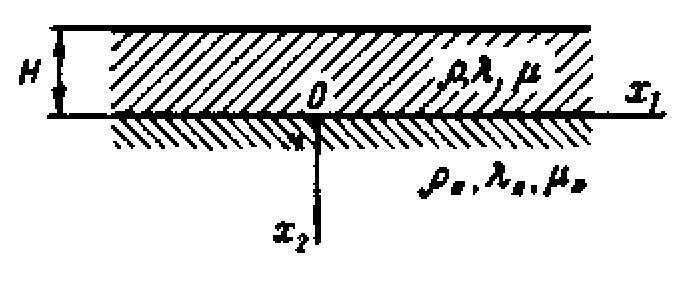
\includegraphics[width=0.5\textwidth]{png/waves-analytics/love-wave.png}}
\caption{К формированию волны Лява.}
\end{figure}

Пусть граница слоя $x_2 = -H$ свободна от нагрузки. Тогда при $x_2 = -H$ верно
\begin{equation}
\sigma_{22} = \sigma_{12} = \sigma_{23} = 0,
\end{equation}

а на границе раздела
\begin{eqnarray}
u_1 = u_1^*, u_2 = u_2^*, u_3 = u_3^*,
\sigma_{22} = \sigma_{22}^*, \sigma_{12} = \sigma_{12}^*, \sigma_{23} = \sigma_{23}^*.
\end{eqnarray}

Потребуем, чтобы при $x_2 \to \infty$, смещения стремились к нулю (граничная волна), причем отличны от нуля были только компоненты $u_3$ и $u_3^*$, не зависящие от $x_3$. Такая волна, если существует, является поперечной. Из уравнения 1.1 получаем:
\begin{eqnarray}
\frac{\partial^2 u_3}{\partial x_1^2} + \frac{\partial^2 u_3}{\partial x_2^2} = \frac{1}{c_2^2} \frac{\partial^2 u_3}{\partial t^2}, \\
\frac{\partial^2 u_3^*}{\partial x_1^2} + \frac{\partial^2 u_3}{\partial x_2^2} = \frac{1}{c_{2*}^2} \frac{\partial^2 u_3^*}{\partial t^2}.
\end{eqnarray}

То есть при $x_2 = -H$ верно $\frac{\partial u_3}{\partial x_2} = 0$, а при $x_2 = 0$ верно $u_3 = u_3^*, \mu\frac{\partial u_3}{\partial x_2} = \mu^*\frac{\partial u_3^*}{\partial x_2}$.

Будем искать такие решения, которые описываются синусоидальным законом:
\begin{eqnarray}
u_3 = f(x_2)e^{iq(x_1-ct)}, \\
u_3 = f_*(x_2)e^{iq(x_1-ct)},
\end{eqnarray}
где $q$ -- заданная частота, $c$ -- неизвестная фазовая скорость. Подставляем в 3.4 и получаем:
\begin{eqnarray}
f^{''} + q^2 \alpha^2 f = 0, \alpha = \sqrt{\frac{c^2}{c_2^2} - 1}, \\
f_*^{''} - q^2 \beta^2 f_* = 0, \beta = \sqrt{1 - \frac{c^2}{c_{*2}^2}}.
\end{eqnarray}

Следовательно
\begin{eqnarray}
f(x_2) = A\sin{\alpha q x_2} + B\cos{\alpha q x_2}, \\
f_*(x_2) = Ce^{-\beta q x_2} + C_1e^{\beta q x_2}.
\end{eqnarray}

Для ограниченности решения $f_*(x_2)$ следует принять $С_1 = 0$, тогда $f_*(x_2) = Ce^{-\beta q x_2}$. Из граничных условий следует, что $B = C, A = - \frac{\mu_* \beta}{\mu \alpha}C$. В итоге получаем
\begin{eqnarray}
\tg{\alpha qH} = \frac{\mu_* \beta}{\mu \alpha}.
\end{eqnarray}

Отсюда мы можем определить отношение $c/c_2$ как функцию параметров $qH$, $c_2/c_{*2}$, $\mu_*/\mu$.  Тогда окончательные формулы для перемещений имеют вид
\begin{eqnarray}
u_3 = C (\cos{\alpha q x_2} - \frac{\mu_* \beta}{\mu \alpha} \sin{\alpha q x_2}) e^{iq(x_1-ct)},
u_3^* = C e^{-q \beta x_2 + i q (x_1 - ct)}.
\end{eqnarray}

Таким образом, мы получили волну, бегущую в направлении оси $x_1$ со скоростью $с$. Перемещения в волне лежат в плоскости, перпендикулярной направлению их распространения, и параллельны границам слоя. Существенно отметить, что фазовая скорость их зависит от частоты, т.е. эти волны имеют дисперсию. Аналогично волнам Рэлея, волны Лява концентрируются вблизи поверхности раздела. Поэтому они затухают медленнее, чем объемные волны, и могут наблюдаться на значительном удалении от источника.


\subsubsection{Расчёт волн Стоунли}

\todo{Вставить картинки}


\subsubsection{Расчёт контакта независимых тел}

\todo{Слова про то, что отдельные тела - тоже всего лишь контакт}

Для проверки расчета контактных границ и взаимодействия тел был выполнен расчёт задачи об ударе по пластине с явным моделированием пластины и ударника на отдельных сетках.

На графиках (см. рис. \ref{pic:striker_test}) изображены поля скоростей в пластине и ударнике.

\begin{figure}[htp]
\begin{subfigure}[b]{0.5\textwidth}
\centering
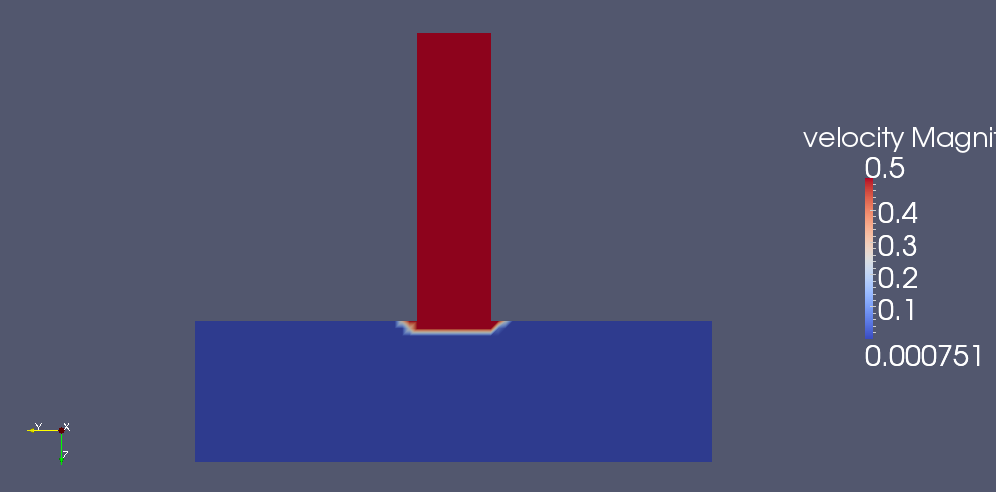
\includegraphics[width=\textwidth]{png/strike-test/both-2d/0001.png}
\caption{1-й временной слой. Начало взаимодействия.}
\end{subfigure}
\begin{subfigure}[b]{0.5\textwidth}
\centering
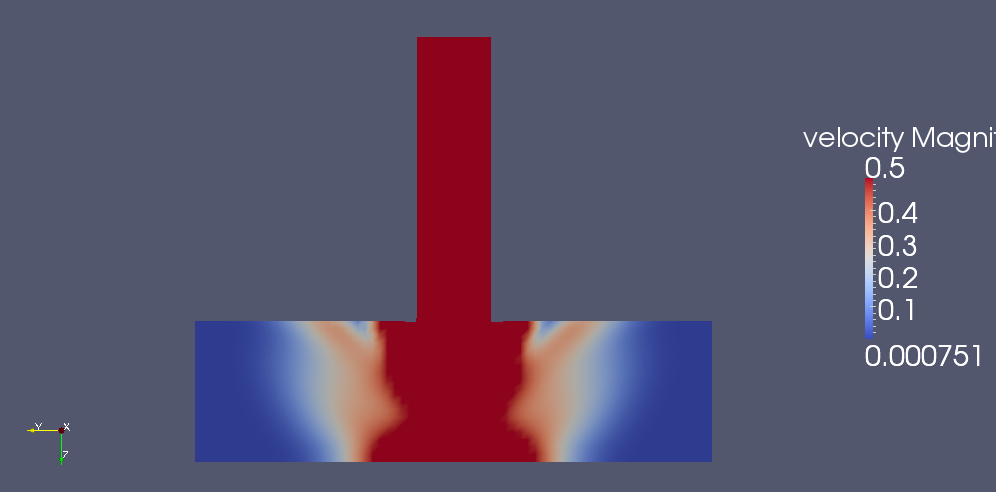
\includegraphics[width=\textwidth]{png/strike-test/both-2d/0040.png}
\caption{40-й временной слой. Отражение волны от тыльной поверхности пластины.}
\end{subfigure}
\begin{subfigure}[b]{0.5\textwidth}
\centering
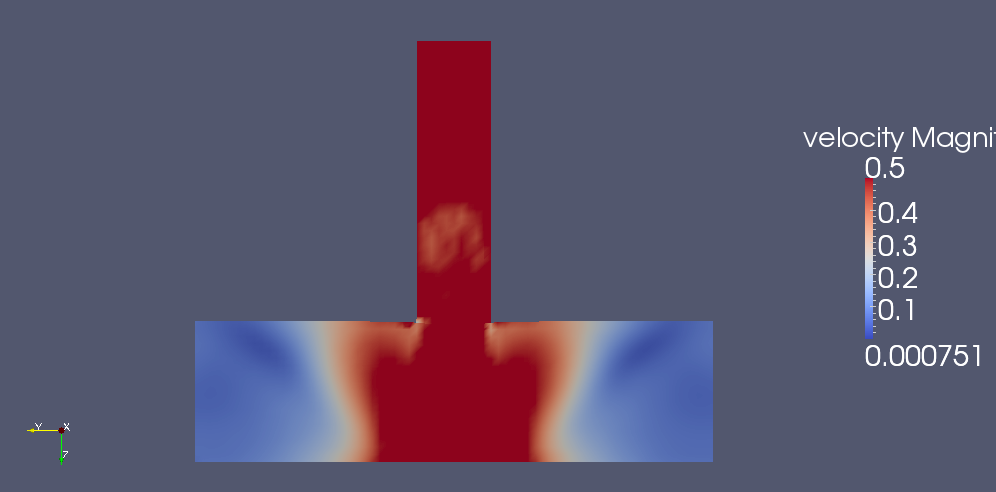
\includegraphics[width=\textwidth]{png/strike-test/both-2d/0120.png}
\caption{120-й временной слой. Проникновение отражённой волны в ударник.}
\end{subfigure}
\begin{subfigure}[b]{0.5\textwidth}
\centering
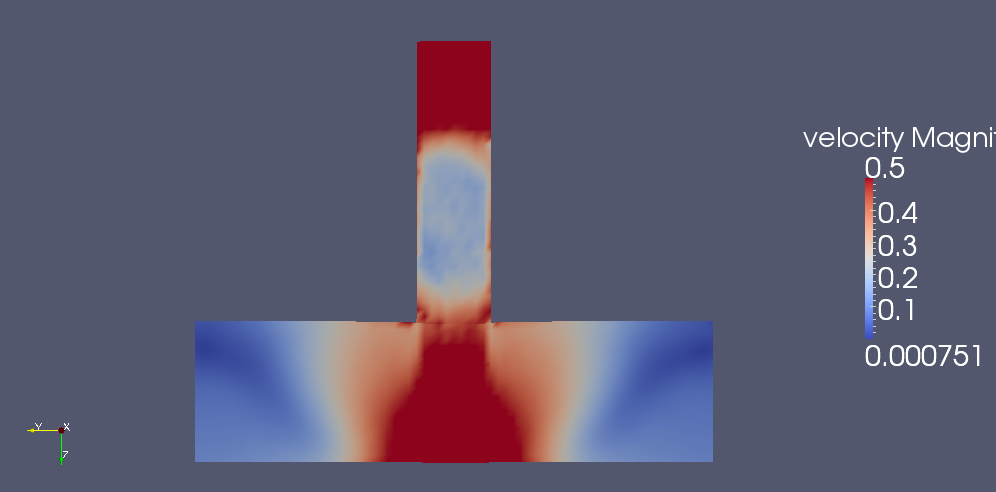
\includegraphics[width=\textwidth]{png/strike-test/both-2d/0160.png}
\caption{160-й временной слой. Нижняя половина ударника остановилась.}
\end{subfigure}
\begin{subfigure}[b]{0.5\textwidth}
\centering
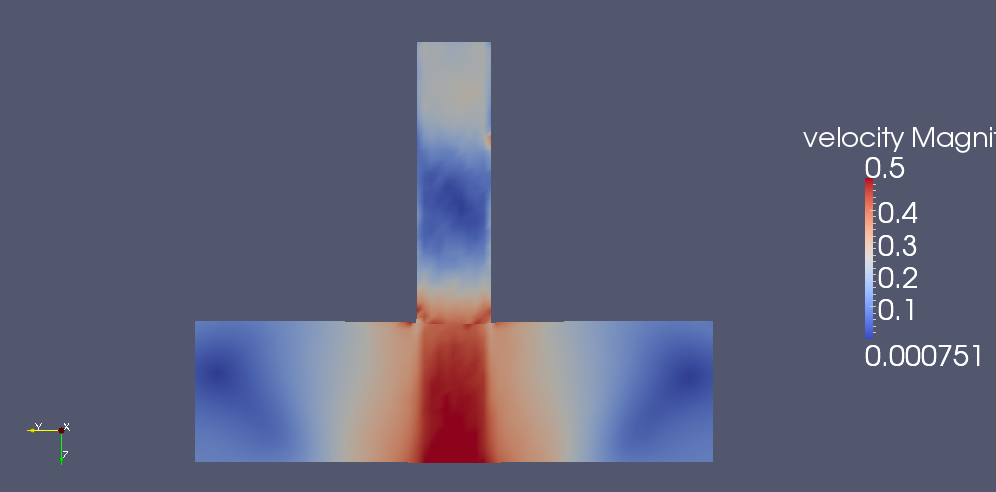
\includegraphics[width=\textwidth]{png/strike-test/both-2d/0200.png}
\caption{200-й временной слой. Полная остановка ударника.}
\end{subfigure}
\begin{subfigure}[b]{0.5\textwidth}
\centering
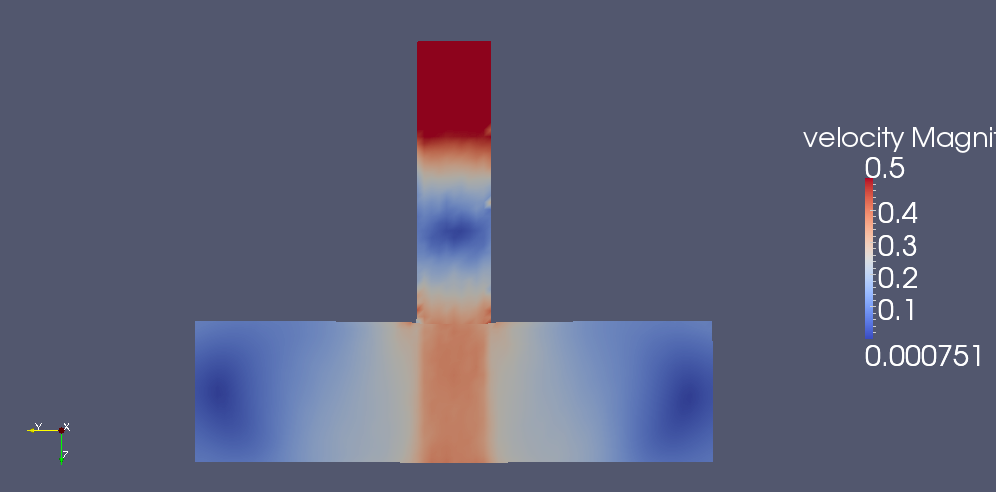
\includegraphics[width=\textwidth]{png/strike-test/both-2d/0240.png}
\caption{240-й временной слой. Начало отскока ударника.}
\end{subfigure}
\caption{Задача контакта двух независимых тел. Цветом изображен модуль скорости.}
\label{pic:striker_test}
\end{figure}

\clearpage
\newpage


\subsection{Генерация волн разных типов}

При численном эксперименте мы можем смоделировать любой тип волны с любым видом ее фронта, задав соответствующие начальные условия. Однако для сравнения с вещественным экспериментом более удобно моделировать волновые процессы в постановке, приближенной к реальной. Чаще всего это означает, что берется невозмущенная среда конечной протяженности, и задается протяженное во времени возмущение на границе.

В 1904 году Лэмб дал точное решение задачи, в которой источник возмущения действовал как импульс, приложенный к участку свободной границы твердого полупространства по нормали к ней. При таком воздействии мы наблюдаем три волновых фронта: продольная волна со сферическим фронтом, поперечная волна со сферическим фронтом и «окном» на нормали к поверхности, волна Рэлея. На данный момент термин "задача Лэмба" часто относят к более общему случаю произвольного источника в среде с одной границей.

Поперечные и продольные волны с прямолинейным фронтом, а также их отражение от свободной границы и преломление на контакте, удобно рассматривать при воздействии на более широкую область, чем в задаче Лэмба. Если брать достаточно большую область воздействия и далеко относить границы моделируемого тела, то возмущения на границах за время моделирования не успеют дойти до интересующего нас участка.

Генерация волн Рэлея и Лэмба может производиться большим количеством разных способов. Они достаточно внимательно исследуются в технике, особенно в задачах ультразвуковой дефектоскопии. Заметим, что при моделировании можно обойтись более простыми методами: например, прямоугольный импульс, аналогичный задаче Лэмба. Объемные волны, «паразитные» по отношению к изучению поверхностных волн, могут быть легко отсечены после расчета.

\clearpage
\newpage


\subsection{Связь волновых процессов с разрушением}

\todo{Ссылки на критерии} - раздел \ref{sec:destruction_models}

Для тестирования работы критериев разрушения был проведен расчет соударения ударника и монолитной преграды (см. рис. \ref{pic:destruction_test}). Область наибольшей концентрации сжимающих и сдвиговых напряжений локализуется в месте удара и имеет характерные размеры порядка размера ударника. Растягивающие напряжения действуют как в области удара (на этапе отскока), так и в тыльных областях ударника и пластины. Сдвиговые напряжения, помимо области удара, образуют откольный конус с тыльной стороны пластины. Распределение сдвиговых напряжений и напряжения Мизеса качественно совпадают.

\begin{figure}[htp]
\centering
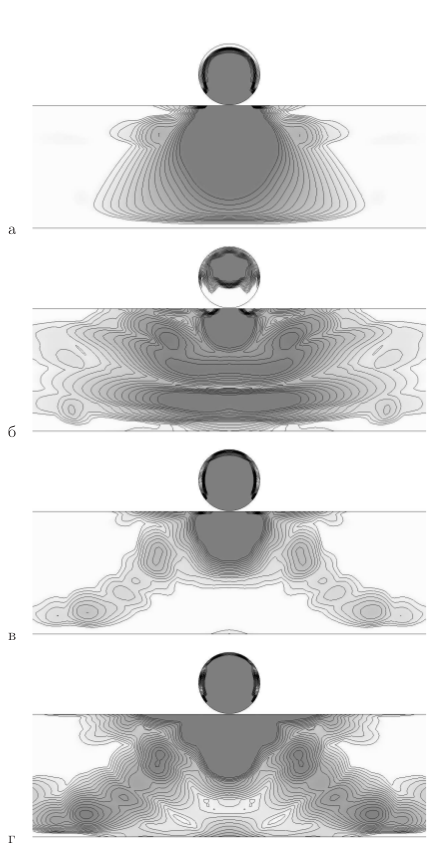
\includegraphics[width=0.45\textwidth]{png/destruction_test.png}
\caption{Тестирование критериев разрушения: а - сжимающие напряжения, б - растягивающие напряжения, в - сдвиговые напряжения, г – приведенные напряжения (критерий Мизеса).}
\label{pic:destruction_test}
\end{figure}

\clearpage
\newpage


\subsection{Расчёт многослойной конструкции}

При расчёте задачи о непробивающем ударе по многослойной преграде использовались
данные из табл. \ref{tbl:subpackage}. В табл. \ref{tbl:subpackage_2} приведены
безразмерные величины, использовавшиеся в расчёте.
\begin{table}[h]
\centering
\begin{tabular}{|c|c|c|c|}
\hline
Слой & $\rho$ & $\lambda$ & $\mu$  \\
\hline
Эпоксидная смола & 1.25 & 1440 & 960 \\
Субпакет & 1.25 & 4620 & 3080 \\
\hline
\end{tabular}
\caption{Безразмерные характеристики слоёв.}
\label{tbl:subpackage_2}
\end{table}

Давление в зоне воздействия ударника задавалось равным 50 МПа (50 единиц в безразмерных величинах).

На графиках (см. рис. \ref{pic:multilayer_init}-\ref{pic:multilayer_Rayleigh_2})
изображены результаты численного расчёта задачи.
На рис. \ref{pic:multilayer_b1}-\ref{pic:multilayer_b3} изображен процесс
прохождения волны через границы раздела двух слоёв. Несмотря на то, что
конструкция состоит из пяти слоёв, волновая картина имеет весьма сложный
вид. На рис. \ref{pic:multilayer_b1}-\ref{pic:multilayer_b3} видны различные
виды волн: волна, созданная начальным возмущением, отраженные от границ волны и
волны, распространяющиеся вдоль границы раздела. Последние, так называемые волны
Рэлея (см. рис. \ref{pic:multilayer_Rayleigh_1}-\ref{pic:multilayer_Rayleigh_2}), 
представляют особый интерес. Появление таких волн в композитных материалах
ожидаемо, но аналитических расчётов, подтверждающих их наличие, на данный момент
нет. Рэлеевские волны формируются на границе раздела двух неоднородных сред и
распространяются вдоль этой границы. Такие волны можно наблюдать, например, в фундаментах
зданий во время землетрясений. Из-за своей низкой частоты, большой
амплитуды и длительного воздействия именно рэлеевские волны наносят наибольший
ущерб зданиям после сейсмической активности. Обнаружение этих волн в композитных
материалах позволяет сделать предположение о том, что области наибольших
напряжений, а, следовательно, и области потери прочности будут сосредоточены
вдоль границ раздела слоёв.

Полученные результаты численного моделирования хорошо согласуются с теоретическими данными,
а также интересны с практической точки зрения. В связи с этим 
дальнейшее исследование волновой картины в композиционных
материалах описанным в работе методом представляет серьёзный научный интерес,
так как может дать ответ на вопрос о том, как ведут себя такие материалы при
непробивающих ударах.
\begin{figure}[htp]
\centering
\includegraphics[width=\textwidth]{png/v-0001.png}
\caption{Начальное возмущение. На рисунке цветом изображены модули скоростей в
двух взаимно перпендикулярных срезах.}
\label{pic:multilayer_init}
\end{figure}
\begin{figure}[htp]
\centering
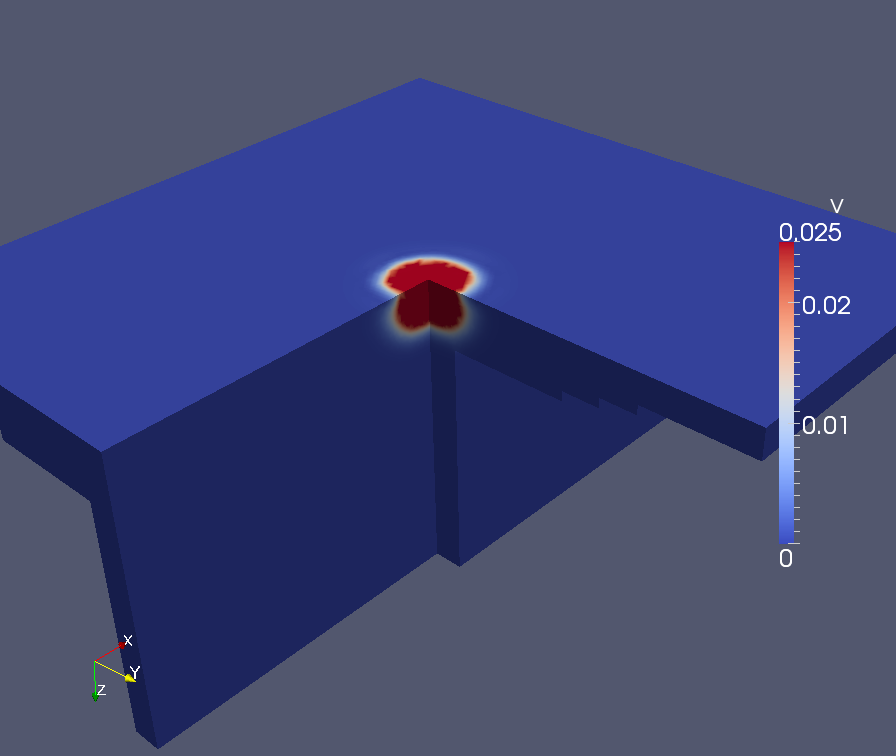
\includegraphics[width=\textwidth]{png/v-0003.png}
\caption{Отражение от первой границы. На рисунке цветом изображены модули скоростей в
двух взаимно перпендикулярных срезах.}
\label{pic:multilayer_b1}
\end{figure}
\begin{figure}[htp]
\centering
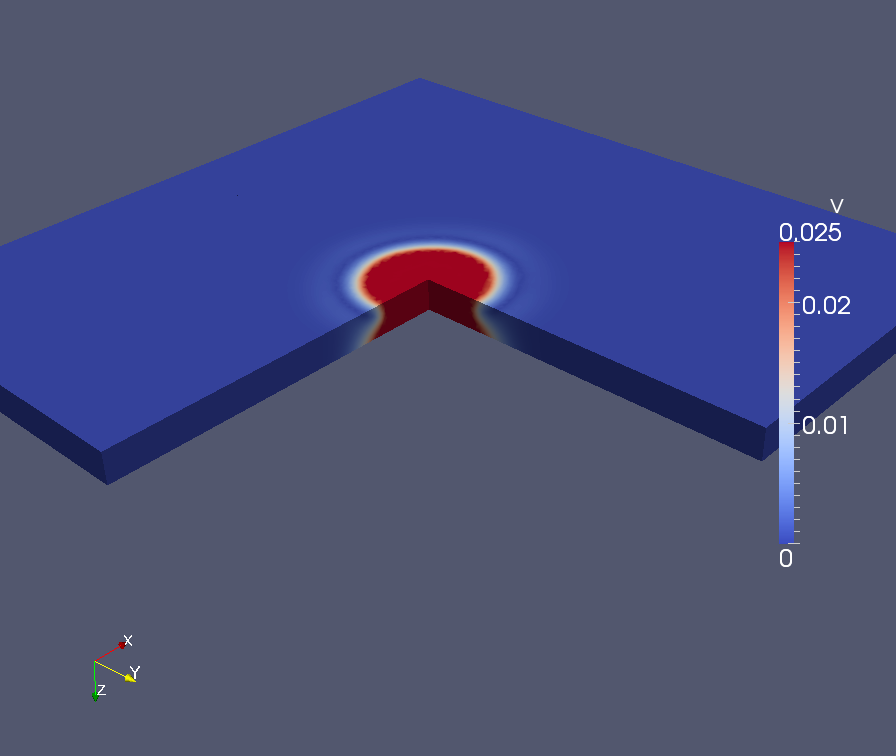
\includegraphics[width=\textwidth]{png/v-0007.png}
\caption{Отражение от второй границы. На рисунке цветом изображены модули скоростей в
двух взаимно перпендикулярных срезах.}
\label{pic:multilayer_b2}
\end{figure}
\begin{figure}[htp]
\centering
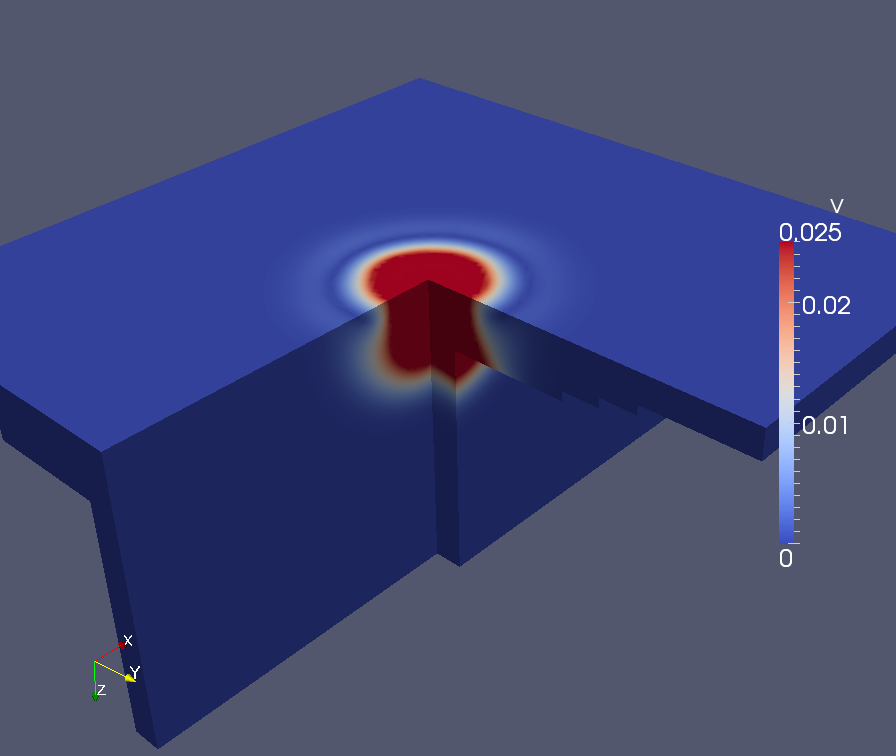
\includegraphics[width=\textwidth]{png/v-0009.png}
\caption{Отражение от третьей границы. На рисунке цветом изображены модули скоростей в
двух взаимно перпендикулярных срезах.}
\label{pic:multilayer_b3}
\end{figure}
\begin{figure}[htp]
\centering
\includegraphics[width=\textwidth]{png/v-0013.png}
\caption{Формирование волны Рэлея. На рисунке цветом изображены модули скоростей
в срезе, перпендикулярном оси x, а стрелками обозначены поля скоростей.}
\label{pic:multilayer_Rayleigh_1}
\end{figure}
\begin{figure}[htp]
\centering
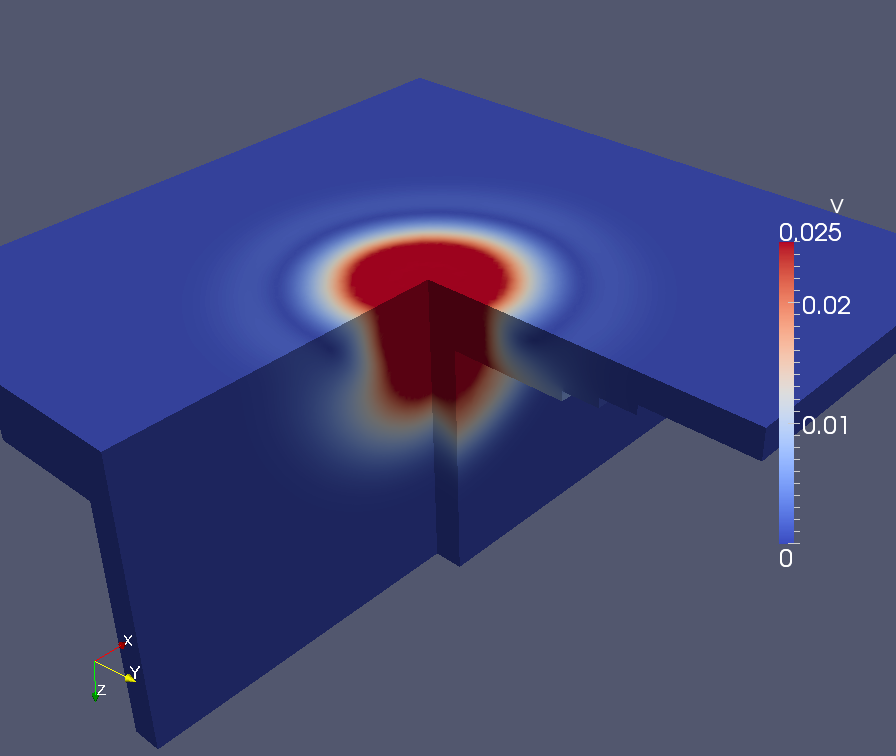
\includegraphics[width=\textwidth]{png/v-0016.png}
\caption{Распространение волны Рэлея. На рисунке цветом изображены модули скоростей
в срезе, перпендикулярном оси x, а стрелками обозначены поля скоростей.}
\label{pic:multilayer_Rayleigh_2}
\end{figure}

\clearpage
\newpage


\section{Низкоскоростной удар по композитной конструкции}

В данном разделе приведены результаты численного моделирования низкоскоростного
удара по композитной конструкции.

\subsection{Общая постановка}

Рассматривается задача о динамическом нагружении элемента композитной обшивки крыла самолёта. На рис.
\ref{pic:construction} приведена схема строения обшивки и силового кессона
крыла, выполненных из композиционных материалов. Обшивка толщиной 6.5~мм состоит 
из 3 композитных субпакетов, стрингер толщиной 13~мм -- из 6 аналогичных субпакетов. Каждый субпакет
состоит из 11 монослоёв со взаимной ориентацией субпакетов при укладке 
45/0/-45/0/0/90/0/0/-45/0/45. Каждый монослой имеет следующий состав: 60\% -- 
ориентированные длинные углепластиковые волокна; 40\% -- матрица
(эпоксидная смола). 

\begin{figure}[h]
\center{\includegraphics[width=\textwidth]{png/construction.png}}
\caption{Обшивка и силовой кессон крыла.}
\label{pic:construction}
\end{figure}

Низкоскоростной удар (от метров в секунду до десятков метров в секунду) 
как правило не приводит к пробиванию и разрушению композитной панели. Однако, 
характеристики конструкции значительно ухудшаются, вплоть до полной непригодности к 
дальнейшей эксплуатации. Это связано с внутренними повреждениями и разрушениями 
в композитном материале. Так, многослойные материалы после нагрузок могут заметно 
терять прочность даже при отсутствии видимых поврежедний.
Это обусловлено появлением внутренних микротрещин, которые впоследствии, объединяясь,
превращаются в макротрещины. Возникающие после нагрузки повреждения
материала могут быть визуально не заметны, хотя делают образец непригодным к
дальнейшему использованию.

Сложное внутреннее строение и многоуровневость структуры композитных материалов вносят несколько 
принципиальных факторов, влияющих на их прочностные свойства.

\begin{itemize}

\item Динамическое воздействие по конструкции вызывает в ней распространение упругих и пластических волн 
нагрузки. В случае композитного материала множественные переотражения волн от внутренних контактных 
границ формируют сложную волновую картину. Интерференция большого количества 
прямых, отражённых и преломлённых волн определяет итоговые области максимальных нагрузок в конструкции. 
Таким образом, внутреннее строение композита влияет на то, где будут локализованы области 
повреждений различных видов.

\item Наличие микроструктуры композита (уровень отдельных волокон в матрице) приводит к появлению зон 
концентрации напряжений. В результате могут заметно снижаться предельные значения напряжений, которые 
выдерживают матрица и волокна в составе композитной конструкции, по сравнению с аналогичными значениями
для изотропных образцов из тех же материалов.

\end{itemize}

В связи с приведёнными фактами одной из актуальных прикладных задач, связанных с прочностными испытаниями 
композитных материалов, является задача о получении волновой картины в образце после
непробивающего удара. 

В эксперименте по непробивающему воздействию на обшивку нагрузка создается 
стальным ударником диаметром 25.4~мм. Характерный пример профиля нагрузки 
при испытаниях приведен на рис. \ref{pic:loadprofile}.
\begin{figure}[h]
\center{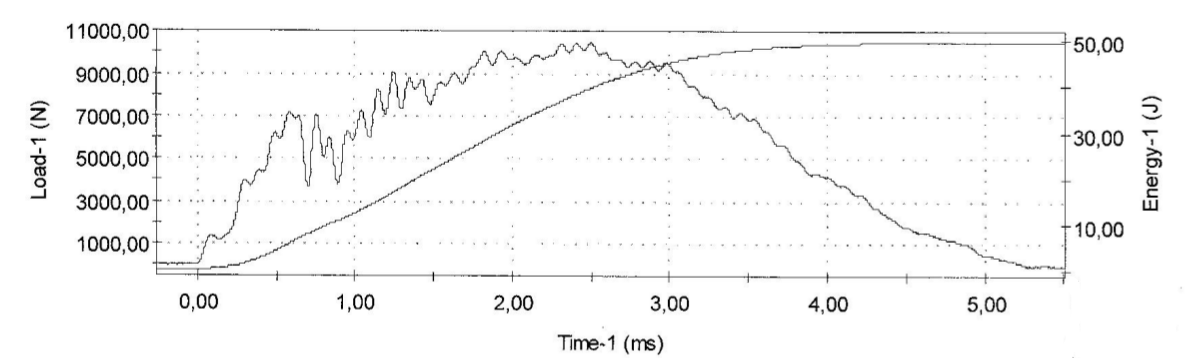
\includegraphics[width=\textwidth]{png/load-profile.png}}
\caption{Пример профиля нагрузки на обшивку крыла при испытаниях.}
\label{pic:loadprofile}
\end{figure}

Ввиду большой вычислительной сложности при моделировании подобной конструкции с 
точностью до отдельного волокна, а также из-за многообразия протекающих процессов, 
полная задача декомпозируется на ряд подзадач. В данном разделе рассматривается задача о получении
волновой картины в элементе композитной обшивки крыла в следующем приближении:
\begin{itemize}
\item конструкция состоит из композитных субпакетов, сооединённых эпоксидной смолой;
\item структура задаётся до уровня отдельного субпакета, монослои в расчёте не выделяются.
\end{itemize}

В данном приближении характеристики субпакетов принимаются равными характеристикам монослоёв, из которых они составлены. 
Анизотропия ниже уровня субпакета, обусловленная укладкой монослоёв внутри субпакета, не рассматривается. Характеристики материалов приведены в табл. \ref{tbl:subpackage} и \ref{tbl:max_stresses}.

\begin{table}
\centering
\begin{tabular}{|c|c|c|c|c|c|c|c|}
\hline
Материал & E, ГПа & $\nu$ & $\rho$, кг/м$^{3}$ & $\lambda$, ГПа & $\mu$, ГПа &
$c_p$, м/с & $c_s$, м/с \\
\hline
Монослой (субпакет) & 8.5 & 0.32 & 1580 & 5.72 & 3.22 & 2775 & 1425 \\
Эпоксидная смола & 2.5 & 0.30 & 1250 & 1.44 & 0.96 & 1640 & 876 \\
Сталь & 200 & 0.28 & 7800 & 99.43 & 78.13 & 5725 & 3165 \\
\hline
\end{tabular}
\caption{Упругие характеристики слоёв и ударника.}
\label{tbl:subpackage}
\end{table}

\begin{table}
\centering
\begin{tabular}{|c|c|}
\hline
Тип нагрузки & Предельно допустимая нагрузка, МПа \\
\hline
Растяжение вдоль волокон & 2630 \\
Сжатие вдоль волокон & 1530 \\
Растяжение поперёк волокон & 86 \\
Сжатие поперёк волокон & 213 \\
Сдвиг & 112 \\
\hline
\end{tabular}
\caption{Прочностные характеристики монослоёв.}
\label{tbl:max_stresses}
\end{table}

Были проведены расчеты для двух постановок эксперимента - удар по отдельному элементу обшивки и удар по элементу обшивки со стрингером.

\clearpage
\newpage


\subsection{Удар по элементу обшивки}

Вид расчетной области приведен на рис. \ref{pic:wing_only_scene}. Часть расчётной сетки показана на рис. \ref{pic:wing_mesh_sample}. Характеристики материалов приведены в табл. \ref{tbl:subpackage} и \ref{tbl:max_stresses}. Скорость ударника в обоих расчётах составляет 6 м/с. На рис. \ref{pic:pkm_experiment_v3d_wing_only} показана общая форма полученного трёхмерного возмущения в конструкции

\begin{figure}[htp]
\center{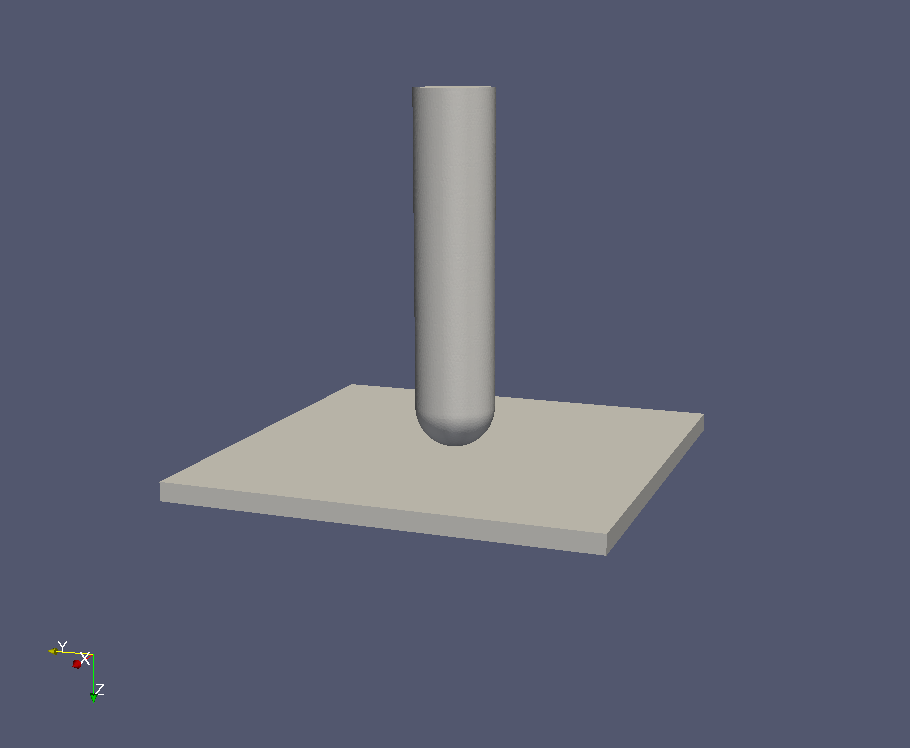
\includegraphics[width=0.75\textwidth]{png/pkm-experiment/wing-only/scene.png}}
\caption{Удар по элементу обшивки. Вид расчетной области.}
\label{pic:wing_only_scene}
\end{figure}

\begin{figure}[htp]
\center{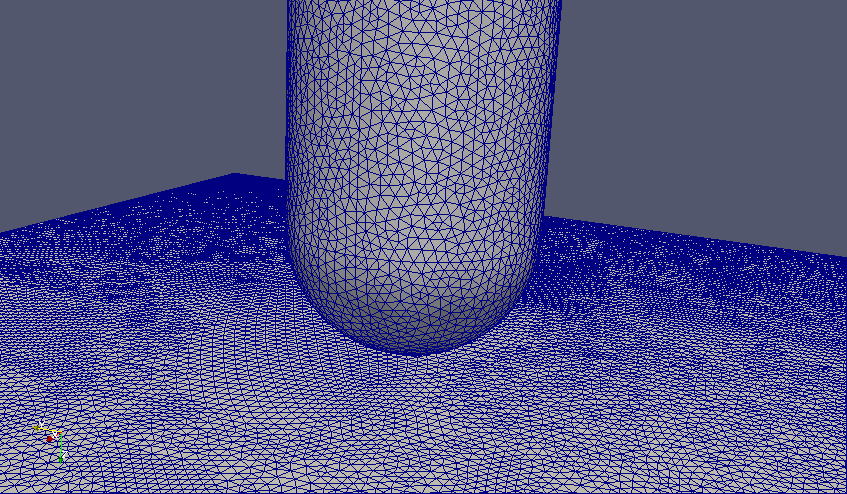
\includegraphics[width=0.75\textwidth]{png/pkm-experiment/mesh.png}}
\caption{Расчётная сетка. Поверхностная сетка в элементе крыла и в ударнике в районе места удара.}
\label{pic:wing_mesh_sample}
\end{figure}

\begin{figure}[htp]
\begin{subfigure}[b]{0.5\textwidth}
\centering
\includegraphics[width=\textwidth]{png/pkm-experiment/wing-only/wave-3d/v-0001.png}
\caption{0.5 мкс}
\end{subfigure}
\begin{subfigure}[b]{0.5\textwidth}
\centering
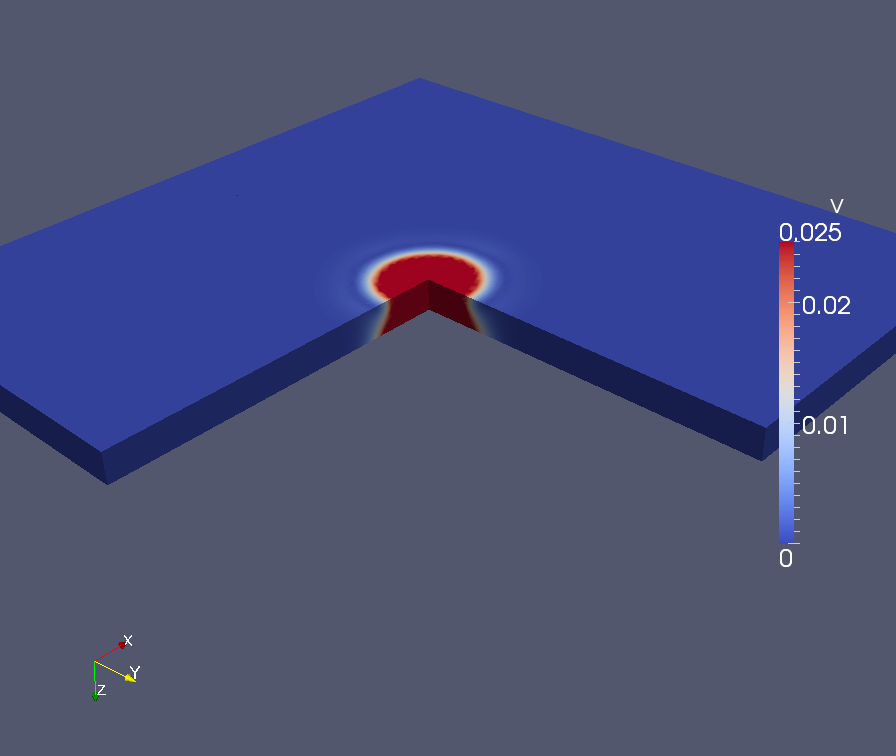
\includegraphics[width=\textwidth]{png/pkm-experiment/wing-only/wave-3d/v-0005.png}
\caption{3.0 мкс}
\end{subfigure}
\begin{subfigure}[b]{0.5\textwidth}
\centering
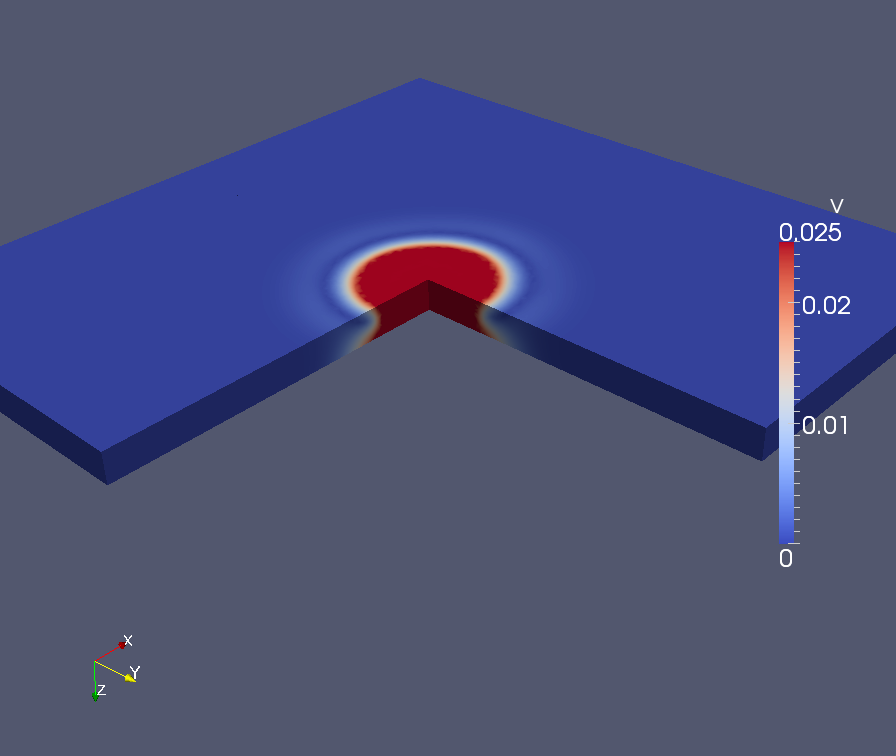
\includegraphics[width=\textwidth]{png/pkm-experiment/wing-only/wave-3d/v-0009.png}
\caption{5.5 мкс}
\end{subfigure}
\begin{subfigure}[b]{0.5\textwidth}
\centering
\includegraphics[width=\textwidth]{png/pkm-experiment/wing-only/wave-3d/v-0013.png}
\caption{8.0 мкс}
\end{subfigure}
\begin{subfigure}[b]{0.5\textwidth}
\centering
\includegraphics[width=\textwidth]{png/pkm-experiment/wing-only/wave-3d/v-0017.png}
\caption{10.5 мкс}
\end{subfigure}
\begin{subfigure}[b]{0.5\textwidth}
\centering
\includegraphics[width=\textwidth]{png/pkm-experiment/wing-only/wave-3d/v-0021.png}
\caption{13.0 мкс}
\end{subfigure}
\caption{Распространение возмущений в элементе обшивки. Общая картина. Цветом показан модуль скорости.}
\label{pic:pkm_experiment_v3d_wing_only}
\end{figure}


\clearpage
\newpage


\subsection{Удар по элементу обшивки со стрингером}

Вид расчетной области приведен на рис. \ref{pic:wing_stringer_scene}. Часть расчётной сетки показана на рис. \ref{pic:wing_mesh_sample}. Характеристики материалов приведены в табл. \ref{tbl:subpackage} и \ref{tbl:max_stresses}. Скорость ударника в обоих расчётах составляет 6 м/с. На рис. \ref{pic:pkm_experiment_v3d_wing_stringer} показана общая форма полученного трёхмерного возмущения в конструкции

\begin{figure}[htp]
\center{\includegraphics[width=0.75\textwidth]{png/pkm-experiment/wing-stringer/scene.png}}
\caption{Удар по элементу обшивки со стрингером. Вид расчетной области.}
\label{pic:wing_stringer_scene}
\end{figure}

\begin{figure}[htp]
\begin{subfigure}[b]{0.5\textwidth}
\centering
\includegraphics[width=\textwidth]{png/pkm-experiment/wing-stringer/wave-3d/v-0001.png}
\caption{0.5 мкс}
\end{subfigure}
\begin{subfigure}[b]{0.5\textwidth}
\centering
\includegraphics[width=\textwidth]{png/pkm-experiment/wing-stringer/wave-3d/v-0005.png}
\caption{3.0 мкс}
\end{subfigure}
\begin{subfigure}[b]{0.5\textwidth}
\centering
\includegraphics[width=\textwidth]{png/pkm-experiment/wing-stringer/wave-3d/v-0009.png}
\caption{5.5 мкс}
\end{subfigure}
\begin{subfigure}[b]{0.5\textwidth}
\centering
\includegraphics[width=\textwidth]{png/pkm-experiment/wing-stringer/wave-3d/v-0013.png}
\caption{8.0 мкс}
\end{subfigure}
\begin{subfigure}[b]{0.5\textwidth}
\centering
\includegraphics[width=\textwidth]{png/pkm-experiment/wing-stringer/wave-3d/v-0017.png}
\caption{10.5 мкс}
\end{subfigure}
\begin{subfigure}[b]{0.5\textwidth}
\centering
\includegraphics[width=\textwidth]{png/pkm-experiment/wing-stringer/wave-3d/v-0021.png}
\caption{13.0 мкс}
\end{subfigure}
\caption{Распространение возмущений в элементе обшивки и стрингере. Общая картина. Цветом показан модуль скорости.}
\label{pic:pkm_experiment_v3d_wing_stringer}
\end{figure}

\clearpage
\newpage

\subsection{Анализ волновой картины для обоих постановок}

На рис. \ref{pic:pkm_experiment_stress_begin} - \ref{pic:pkm_experiment_stress_end} показано распространение напряжений в зоне удара как для отдельного элемента обшивки, так и для конструкции со стрингером.

В начальный момент (рис. \ref{pic:pkm_experiment_stress_begin}) фронт волны близок к сферическому, геометрические размеры определяются площадью контакта между ударником и пластиной, а точная форма -- строением элемента обшивки.

К концу данной стадии соударения волна сжатия проходит элемент обшивки. Для постановки без стрингера начинается отражение волны от противоположной свободной границы, фронт очевидным образом перестает быть сферическим, полная волновая картина в образце представляет сумму падающей и отражённой волн. Для постановки со стрингером начинается проникновение волны в стрингер. В данной области субпакеты, составляющие стрингер, ориентированы параллельно субпакетам обшивки (см. рис. \ref{pic:construction}), поэтому форма фронта не меняется.

\begin{figure}[htp]
\begin{subfigure}[b]{0.5\textwidth}
\centering
\includegraphics[width=\textwidth]{png/pkm-experiment/wing-only/wave/syy-0001.png}
\caption{0.5 мкс}
\end{subfigure}
\begin{subfigure}[b]{0.5\textwidth}
\centering
\includegraphics[width=\textwidth]{png/pkm-experiment/wing-stringer/wave/syy-0001.png}
\caption{0.5 мкс}
\end{subfigure}
\begin{subfigure}[b]{0.5\textwidth}
\centering
\includegraphics[width=\textwidth]{png/pkm-experiment/wing-only/wave/syy-0003.png}
\caption{3.0 мкс}
\end{subfigure}
\begin{subfigure}[b]{0.5\textwidth}
\centering
\includegraphics[width=\textwidth]{png/pkm-experiment/wing-stringer/wave/syy-0003.png}
\caption{3.0 мкс}
\end{subfigure}
\caption{Начальный момент удара. Цветом показаны напряжения. Синий соответствует сжатию, красный -- растяжению.}
\label{pic:pkm_experiment_stress_begin}
\end{figure}

На следующей стадии соударения (рис. \ref{pic:pkm_experiment_stress_middle}) в постановке без стрингера формируется волна растяжения, отражённая от свободной границы (рис. \ref{pic:pkm_experiment_stress_middle}а). Также заметно более слабая волна растяжения формируется в области, непосредственно прилежащей к зоне контакта (рис. \ref{pic:pkm_experiment_stress_middle}c и \ref{pic:pkm_experiment_stress_middle}d).

Для постановки со стрингером исходная волна сжатия еще не достигла свободной поверхности, от которой могло бы произойти заметное отражение. В результате наблюдаются менее выраженные области растяжения (рис. \ref{pic:pkm_experiment_stress_middle}b и \ref{pic:pkm_experiment_stress_middle}d), обусловленные волной растяжения в зоне контакта и относительно слабыми волнами, отражёнными от границ между субпакетами. На рис. \ref{pic:pkm_experiment_stress_middle}d видно изменение формы фронта первончальной волны. Это связано с тем, что волна дошла до зоны, где субпакеты стрингера ориентированы перпендикулярно субпакетам обшивки (см. рис. \ref{pic:construction}).

\begin{figure}[htp]
\begin{subfigure}[b]{0.5\textwidth}
\centering
\includegraphics[width=\textwidth]{png/pkm-experiment/wing-only/wave/syy-0005.png}
\caption{5.5 мкс}
\end{subfigure}
\begin{subfigure}[b]{0.5\textwidth}
\centering
\includegraphics[width=\textwidth]{png/pkm-experiment/wing-stringer/wave/syy-0005.png}
\caption{5.5 мкс}
\end{subfigure}
\begin{subfigure}[b]{0.5\textwidth}
\centering
\includegraphics[width=\textwidth]{png/pkm-experiment/wing-only/wave/syy-0007.png}
\caption{8.0 мкс}
\end{subfigure}
\begin{subfigure}[b]{0.5\textwidth}
\centering
\includegraphics[width=\textwidth]{png/pkm-experiment/wing-stringer/wave/syy-0007.png}
\caption{8.0 мкс}
\end{subfigure}
\caption{Проникновение волны в конструкцию. Цветом показаны напряжения. Синий соответствует сжатию, красный -- растяжению.}
\label{pic:pkm_experiment_stress_middle}
\end{figure}

В дальнейшем в постановке без стрингера наблюдается многократное переотражение волн от параллельных свободных поверхностей и внутренних контактных границ. Одновременно с этим амплитуда волн затухает по мере удаления от места удара. Интерференция всех волн формирует распределение сжатий и растяжений (рис. \ref{pic:pkm_experiment_stress_middle}a, \ref{pic:pkm_experiment_stress_middle}c), характерное для удара по многослойной конструкции.

В постановке со стрингером происходит отражение волны от свободных поверхностей в районе изгиба субпакетов стрингера (рис. \ref{pic:pkm_experiment_stress_middle}b, \ref{pic:pkm_experiment_stress_middle}d). Отражение в целом заметно менее выражено, чем в постановке без стрингера. Это связано как с тем, что волна уже ослаблена отражением от контактных границ, так и геометрией области -- значительная часть энергии волны проходит в стрингер без взаимодействия со свободной границей.


\begin{figure}[htp]
\begin{subfigure}[b]{0.5\textwidth}
\centering
\includegraphics[width=\textwidth]{png/pkm-experiment/wing-only/wave/syy-0009.png}
\caption{10.5 мкс}
\end{subfigure}
\begin{subfigure}[b]{0.5\textwidth}
\centering
\includegraphics[width=\textwidth]{png/pkm-experiment/wing-stringer/wave/syy-0009.png}
\caption{10.5 мкс}
\end{subfigure}
\begin{subfigure}[b]{0.5\textwidth}
\centering
\includegraphics[width=\textwidth]{png/pkm-experiment/wing-only/wave/syy-0011.png}
\caption{13.0 мкс}
\end{subfigure}
\begin{subfigure}[b]{0.5\textwidth}
\centering
\includegraphics[width=\textwidth]{png/pkm-experiment/wing-stringer/wave/syy-0011.png}
\caption{13.0 мкс}
\end{subfigure}
\caption{Проникновение волны в конструкцию. Цветом показаны напряжения. Синий соответствует сжатию, красный -- растяжению.}
\label{pic:pkm_experiment_stress_end}
\end{figure}

\clearpage
\newpage

\subsection{Анализ максимальных напряжений разных типов}

На рис. \ref{pic:pkm_experiment_compression} цветом показаны максимальные значения сжатия в каждой точке конструкции за все время соударения. Сжатия очевидным образом концентрируются в месте удара. Зона максимального сжатия имеет характерный размер порядка диаметра области контакта между ударником и пластиной.

\begin{figure}[htp]
\begin{subfigure}[b]{0.5\textwidth}
\centering
\includegraphics[width=\textwidth]{png/pkm-experiment/wing-only/compression.png}
\caption{Элемент обшивки.}
\end{subfigure}
\begin{subfigure}[b]{0.5\textwidth}
\centering
\includegraphics[width=\textwidth]{png/pkm-experiment/wing-stringer/compression.png}
\caption{Элемент обшивки и стрингер.}
\end{subfigure}
\caption{Максимальные сжатия (по модулю) за всё время соударения.}
\label{pic:pkm_experiment_compression}
\end{figure}

В случае конструкции без стрингера дополнительно видны относительно слабые области сжатия на обратной поверхности элемента обшивки, вызванные волнами, испытавшими два отражения -- первое от противолежащей свободной поверхности, второе от поверхности, по которой приходится удар.

В случае конструкции со стрингером видно заметное проникновение волны сжатия в основание стрингера. Вторичные зоны сжатия выражены значительно слабее, чем без стрингера, из-за большого количества переотражений от внутренних контактных границ.

Амплитуда максимального сжатия совпадает в обоих постановках. Диаметр зоны потенциальных разрушений составляет 16-20 мм.

Отдельно стоит отметить, что в субпакетах элемента обшивки сжатие действует поперёк волокон, а в основании стрингера -- вдоль волокон (см. рис. \ref{pic:construction}). Так как прочность монослоёв на сжатие в направлении волокон почти на порядок больше, чем поперёк них, то основные разрушения в конструкции стоит ожидать в элементе обшивки. В основании стрингера могут быть разрушены участки субпакетов, параллельные обшивке, но разрушение самого стрингера маловероятно.


\clearpage
\newpage

На рис. \ref{pic:pkm_experiment_tension} цветом показаны максимальные значения растяжения в каждой точке конструкции за все время соударения.

\begin{figure}[htp]
\begin{subfigure}[b]{0.5\textwidth}
\centering
\includegraphics[width=\textwidth]{png/pkm-experiment/wing-only/tension.png}
\caption{Элемент обшивки.}
\end{subfigure}
\begin{subfigure}[b]{0.5\textwidth}
\centering
\includegraphics[width=\textwidth]{png/pkm-experiment/wing-stringer/tension.png}
\caption{Элемент обшивки и стрингер.}
\end{subfigure}
\caption{Максимальные растяжения (по модулю) за всё время соударения.}
\label{pic:pkm_experiment_tension}
\end{figure}

В случае конструкции без стрингера растягивающие напряжения выражены достаточно явно. Это связано с многократным переотражением волн в тонкой конструкции при относительно слабом рассеивании и затухании. Волны растяжения от первого и второго отражения имеют значительную амплитуду, что видно на рисунке.

Принципиально, что волны растяжения в обшивке действуют поперёк направления волокон в субпакетах обшивки. Сопротивление монослоёв такому типу нагрузки минимально. Диаметр зоны потенциальных разрушений оказывается заметно больше размеров ударника и составляет около 50 мм

В случае конструкции со стрингером столь ярко выраженные зоны растягивающих напряжений не формируются, так как волна нагрузки большей частью проходит в стрингер, который за счёт этого "разгружает" обшивку. У основания стрингера при отражении от свободных поверхностей формируются две зоны растягивающих напряжений -- в районе изгиба субпакетов стрингера и поперёк стрингера. В изгибе субпакетов напряжения достаточно велики и при этом действуют поперёк направления волокон. В этой зоне можно ожидать появления разрушений. Зона растяжения поперёк стрингера ориентирована таким образом, что нагрузка действует вдоль волокон, которые хорошо выдерживают такую нагрузку. В этой зоне разрушения маловероятны.


\clearpage
\newpage


На рис. \ref{pic:pkm_experiment_shear} цветом показаны максимальные значения сдвиговых напряжений в каждой точке конструкции за все время соударения.

\begin{figure}[htp]
\begin{subfigure}[b]{0.5\textwidth}
\centering
\includegraphics[width=\textwidth]{png/pkm-experiment/wing-only/shear.png}
\caption{Элемент обшивки.}
\end{subfigure}
\begin{subfigure}[b]{0.5\textwidth}
\centering
\includegraphics[width=\textwidth]{png/pkm-experiment/wing-stringer/shear.png}
\caption{Элемент обшивки и стрингер.}
\end{subfigure}
\caption{Максимальные сдвиговые напряжения (по модулю) за всё время соударения.}
\label{pic:pkm_experiment_shear}
\end{figure}

Сдвиговые напряжения локализуются на периферии зоны максимального сжатия. В однородной среде зона максимальных сдвиговых напряжений имеет форму конуса, расходящегося от места удара (см. рис. \ref{pic:destruction_test}). В случае многослойной среды, моделирующей композит, из-за переотражений волн формируется зона, по форме более близкая к колоколу. Вследствие этого характерный размер зоны действия сдвиговых напряжений зависит от толщины пластины.

На качественном уровне картина оказывается одинаковой как для одиночного элемента обшивки, так и для элемента обшивки со стрингером. Количественно размер повреждённой зоны оказывается несколько больше во втором случае из-за большей толщины конструкции в месте удара. Для первой постановки характерный размер зоны составляет 20 мм, для второй -- 25-30 мм.

Во всей области действия максимальных сдвиговых нагрузок структура композита такова, что направление сдвига приходится поперёк волокон. Монослои композита не очень хорошо держат нагрузку такого вида, поэтому разрушения в данной области возможны.


\clearpage
\newpage


На рис. \ref{pic:pkm_experiment_mises} цветом показаны максимальные значения эквивалентного напряжения Мизеса в каждой точке конструкции за все время соударения.

\begin{figure}[htp]
\begin{subfigure}[b]{0.5\textwidth}
\centering
\includegraphics[width=\textwidth]{png/pkm-experiment/wing-only/mises.png}
\caption{Элемент обшивки.}
\end{subfigure}
\begin{subfigure}[b]{0.5\textwidth}
\centering
\includegraphics[width=\textwidth]{png/pkm-experiment/wing-stringer/mises.png}
\caption{Элемент обшивки и стрингер.}
\end{subfigure}
\caption{Максимальное эквивалентное напряжение Мизеса (по модулю) за всё время соударения.}
\label{pic:pkm_experiment_mises}
\end{figure}

Как рассмотрено выше, напряжение Мизеса характеризует девиаторную часть тензора напряжений. Нагрузки такого типа связаны с изменением формы вещества без изменения его объёма. В однородной среде зона максимальных напряжений Мизеса с хорошей точностью совпадает с зоной максимальных сдвиговых напряжений (см. рис. \ref{pic:destruction_test}) и так же как и она имеет форму конуса, хотя и несколько большего и с более ярко выраженным максимумом в точке удара.

Для композита рассматриваемой структуры получено, что характер распределения напряжений Мизеса несколько меняется. Область принимает колоколообразную форму, аналогично сдвиговым напряжениям. Кроме того, значительно более ярко по сравнению с изотропной средой выражен максимум непосредственно в зоне удара.

В постановке без стрингера напряжения Мизеса значительно меньше, чем при наличии стрингера, так как отражения от близкой свободной поверхности быстро компенсируют девиаторную часть нагрузки, переводя её в растяжения.


\clearpage
\newpage

\subsection{Интегральное воздействие и области разрушений}

Для оценки итоговых областей разрушений необходимо учитывать разрушения всех приведённых типов. При этом, как видно из таблицы \ref{tbl:max_stresses}, устойчивость монослоёв при нагрузках разных типов значительно отличается. В качестве интегральной характеристики воздействия использовался параметр

\begin{equation}
\sigma^* = \sum{k_i max(\sigma_i)},
\end{equation}

где суммирование ведётся по типам нагрузки (сжатие, растяжение, сдвиг, изменение формы), $max(\sigma_i)$ -- максимальное значение напряжения данного типа в данной точке за всё время воздействия, $k_i$ -- коэффициент нормировки. Коэффициенты нормировки $k_i$ для напряжений различных типов были выбраны обратно пропорционально пределу прочности монослоёв при нагрузках соответствующего типа. Для упрощения оценки использовались следующие значения: сжатие -- 1, сдвиг и изменение формы -- 2, растяжение -- 3.

Вообще говоря, в случае динамической нагрузки пределы прочности могут заметно отличаться от указанных значений. Соответственно, следует корректировать и вклад напряжений разных типов в итоговое распределение разрушений. Тем не менее, для низкоскоростного удара воспользуемся этими данными.

Интегральная оценка областей потенциального разрушения материала для постановки с отдельным элементом обшивки приведена на рис. \ref{pic:pkm_experiment_wing_only_result}. Размер разрушенной области заметно превышает размер ударника и составляет 50-60 мм. По форме разрушенная область представляет собой цилиндр с утоньшением посередине. Как было показано выше, разрушения на оси удара (10-15 мм от оси симметрии удара) связаны со сжатием и сдвигом. Разрушения в более дальней области (15-30 мм от оси симметрии удара) обусловлены волнами растяжения.


\begin{figure}[htp]
\begin{subfigure}[b]{\textwidth}
\centering
\includegraphics[width=\textwidth]{png/pkm-experiment/wing-only/sum-3d.png}
\caption{Срез через центр элемента параллельно грани.}
\end{subfigure}
\begin{subfigure}[b]{\textwidth}
\centering
\includegraphics[width=\textwidth]{png/pkm-experiment/wing-only/sum.png}
\caption{Сечение через центр элемента параллельно грани.}
\end{subfigure}
\caption{Области разрушений в элементе обшивки.}
\label{pic:pkm_experiment_wing_only_result}
\end{figure}

Интегральная оценка областей потенциального разрушения материала для постановки с элементом обшивки и стрингером приведена на рис. \ref{pic:pkm_experiment_wing_stringer_result}. Размер разрушенной области порядка размера ударника -- 25 мм. По форме разрушенная область представляет собой колокол, уходящий вглубь конструкции. Как было показано выше, разрушения обусловлены сжатием, сдвигом и изменением формы.

Отдельный комментарий необходим относительно отмеченной области разрушения в стрингере. Значения напряжений в данной области действительно достаточно велики, однако воздействие направлено вдоль волокон (см. рис. \ref{pic:construction}. Предел прочности в направлении волокон монослой выдерживает практически на порядок лучше, чем поперёк волокон (\ref{tbl:max_stresses}), поэтому на практике разрушения в стрингере маловероятны.

\begin{figure}[htp]
\begin{subfigure}[b]{\textwidth}
\center
\includegraphics[width=\textwidth]{png/pkm-experiment/wing-stringer/sum-3d.png}
\caption{Срез через центр элемента параллельно грани.}
\end{subfigure}
\begin{subfigure}[b]{\textwidth}
\center
\includegraphics[width=\textwidth]{png/pkm-experiment/wing-stringer/sum.png}
\caption{Сечение через центр элемента параллельно грани.}
\end{subfigure}
\caption{Области разрушений в элементе обшивки и стрингере.}
\label{pic:pkm_experiment_wing_stringer_result}
\end{figure}

Таким образом, в случае динамического воздействия разрушения в конструкции со стрингером оказываются заметно меньше за счёт того, что волны напряжения уходят в стрингер, и это "разгружает" элемент обшивки. Данный факт отдельно интересен в связи с тем, что при статической нагрузке наличие стрингера напротив приводит к концентрации напряжений и более раннему разрушению элемента обшивки.


\clearpage
\newpage

\subsection{Несимметричный удар по конструкции со стрингером}

Дополнительно были выполнены расчёты для несимметричного удара по элементу обшивки со стрингером. Вид расчётной области представлен на рис. \ref{pic:wing_stringer_non_center_scene}. Точка удара в этой постановке смещена от оси прикрепления стрингера на 30 мм перпендикулярно плоскости стрингера. Все остальные параметры объектов без изменений.

\begin{figure}[htp]
\center{\includegraphics[width=0.75\textwidth]{png/pkm-experiment/wing-stringer-non-center/scene.png}}
\caption{Несимметричный удар по элементу обшивки со стрингером. Вид расчетной области.}
\label{pic:wing_stringer_non_center_scene}
\end{figure}

Данная постановка интересна по двум причинам. Во-первых, в ходе эксплуатации композитных изделий следует ожидать по большей части несимметричных ударов. Во-вторых, сравнение результатов воздействия при центральном и нецентральном ударах по конструкции со стрингером позволяет выполнить верификацию полученных результатов и уточнить, какие типы нагрузок преимущественно вызывают разрушения.

Полученные значения максимальных напряжений представлены на рис. \ref{pic:pkm_experiment_non_center}. Распределение максимальных сжатий, сдвигов и напряжений Мизеса хорошо совпадает с аналогичными распределениями для удара по элементу обшивки без стрингера. Этот результат вполне логичен, так как общий вид конструкции тот же -- тонкая пластина, в которой наблюдаются множественные переотражения на малой толщине. Детали геометрии области отличаются -- больше толщина и больше контактных границ, обратная свободная поверхность не плоская. Это влияет на точную форму волновых фронтов, но не меняет принципиальную картину. Стрингер расположен в стороне от зоны удара и не разгружает конструкцию, так как наиболее сильные волны до него не доходят, а диссипация слабых многократно отражённых и преломлённых волн не сказывается на зонах потенциальных разрушений.

\clearpage
\newpage

\begin{figure}[h]
\begin{subfigure}[b]{0.5\textwidth}
\centering
\includegraphics[width=\textwidth]{png/pkm-experiment/wing-stringer-non-center/compression.png}
\caption{Максимальное сжатие (по модулю) за всё время соударения.}
\end{subfigure}
\begin{subfigure}[b]{0.5\textwidth}
\centering
\includegraphics[width=\textwidth]{png/pkm-experiment/wing-stringer-non-center/tension.png}
\caption{Максимальное растяжение (по модулю) за всё время соударения.}
\end{subfigure}
\begin{subfigure}[b]{0.5\textwidth}
\centering
\includegraphics[width=\textwidth]{png/pkm-experiment/wing-stringer-non-center/shear.png}
\caption{Максимальное сдвиговое напряжение (по модулю) за всё время соударения.}
\end{subfigure}
\begin{subfigure}[b]{0.5\textwidth}
\centering
\includegraphics[width=\textwidth]{png/pkm-experiment/wing-stringer-non-center/mises.png}
\caption{Максимальное напряжение Мизеса (по модулю) за всё время соударения.}
\end{subfigure}
\caption{Максимальные нагрузки при нецентральном ударе.}
\label{pic:pkm_experiment_non_center}
\end{figure}

Иначе обстоит дело для волн растяжения -- их распределение принципиально отличается от рассмотренных постановок с центральными ударами.

В рассматриваемой постановке зона контакта ударника и пластины находится напротив края крепления стрингера. Первоначальная волна сжатия отражается как от тыльных поверхностей субпакетов (параллельных внешней поверхности обшивки), так и от кромок субпакетов стрингера (расположенных перпендикулярно к поверхности обшивки). В результате каждого такого отражения формируется волна растяжения. Три такие волны движутся вверх, и три -- вправо. При сложении этих волн формируется итоговая область растягивающих напряжений (рис. \ref{pic:pkm_experiment_non_center}b).

Амплитуда растягивающих напряжений в области края крепления стрингера из-за сложения волн оказывается в 2.5 раза больше, чем значение на тыльной поверхности для конструкции без стрингера. При этом на верхней границе образца растягивающие напряжения оказываются заметно меньше (в 1.5-2 раза) по сравнению с элементом обшивки без стрингера.

Интегральная оценка воздействия и потенциальные зоны разрушения при нецентральном ударе показаны на рис. \ref{pic:pkm_experiment_wing_stringer_non_center_result}. Форма области близка к колоколу, но при этом является достаточно узкой -- её диаметр не превышает диаметра ударника и составляет 20-25 мм.


\begin{figure}[h]
\begin{subfigure}[b]{\textwidth}
\center
\includegraphics[width=\textwidth]{png/pkm-experiment/wing-stringer-non-center/sum-3d.png}
\caption{Срез через центр элемента параллельно грани.}
\end{subfigure}
\begin{subfigure}[b]{\textwidth}
\center
\includegraphics[width=\textwidth]{png/pkm-experiment/wing-stringer-non-center/sum.png}
\caption{Сечение через центр элемента параллельно грани.}
\end{subfigure}
\caption{Области разрушений при нецентральном ударе.}
\label{pic:pkm_experiment_wing_stringer_non_center_result}
\end{figure}


\clearpage
\newpage

\subsection{Сравнение последствий удара для разных постановок}

Основные результаты в части разрушения конструкции представлены в таблице \ref{tbl:destruction_summary}.

\begin{table}
\centering
\begin{tabular}{|c|c|c|}
\hline
Постановка задачи & Диаметр разрушенной области, мм & Чем обусловлено разрушение \\
\hline
Элемент обшивки без стрингера, центральный удар & 50-60 & Сжатие и сдвиг в центральной зоне, растяжение в периферийной зоне \\
Элемент обшивки со стрингером, центральный удар & 25-30 & Сжатие, сдвиг, напряжение Мизеса \\
Элемент обшивки со стрингером, нецентральный удар & 20-25 & Сжатие и сдвиг на внешней поверхности, растяжение на тыльной поверхности \\
\hline
\end{tabular}
\caption{Прочностные характеристики монослоёв.}
\label{tbl:destruction_summary}
\end{table}



\clearpage
\newpage


\section{Взаимодействие падающей волны с поврежденной зоной}

Отдельной задачей является моделирование тела с повреждениями. Данная задача важна при определении последствий повторных ударов по конструкции. В этом случае конструкция может уже не являться сплошной, в ней содержатся трещины, зоны раздробленного материала и другие повреждения.

Реологические характеристики поврежденных зон заметно отличаются от характеристик окружающего материала. С одной стороны, это приводит к тому, что остаточная прочность конструкции может заметно снизиться по сравнению с первоначальной. С другой стороны, появившиеся неоднородности оказывают влияние на волновую картину при повторных воздействиях и могут заметно ее искажать.

В данной работе рассматривается взаимодействие волны нагрузки с зоной разрушенного материала. Расчетная область с сеткой представлена на рис. \ref{pic:crack_mesh}. Разрушенная зона и окружающий неповрежденный материал моделируются явным образом на отдельных сетках. На контактной границе стоит условие полного слипания.

\begin{figure}[htp]
\center{\includegraphics[width=0.5\textwidth]{png/wave-around-crack/mesh.png}}
\caption{Расчетная область с сеткой.}
\label{pic:crack_mesh}
\end{figure}

Материал исходной среды принимается хрупким, что соответствует эпоксидной матрице композита. В этом случае разрушенная зона представляет собой раздробленный материал. Через зону разрушения такого типа продольные волны проходят медленнее, чем через окружающую неповрежденную среду, а поперечные волны практически не проходят. В связи с этим раздробленная зона моделируется изменением характеристик материала - параметр $\lambda$ уменьшается в два раза, параметр $\mu$ принимается близким к нулю. 

Характеристики исходного и разрушенного материала приведены в табл. \ref{tbl:crack}
\begin{table}
\centering
\begin{tabular}{|c|c|c|c|c|c|}
\hline
Материал & $\rho$, кг/м$^{3}$ & $\lambda$, ГПа & $\mu$, ГПа &
$c_p$, м/с & $c_s$, м/с \\
\hline
Матрица (эпоксидная смола) & 1250 & 1.44 & 0.96 & 1640 & 876 \\
Разрушенная матрица & 1250 & 0.73 & 0.01 & 775 & 89 \\
\hline
\end{tabular}
\caption{Характеристики исходного и разрушенного материала.}
\label{tbl:crack}
\end{table}

Разрушенная область имеет малые размеры по сравнению с полной конструкцией, что требует использовать в ней крайне мелкую сетку. Использование сетки такой же мелкости для расчета всего окружающего материала ведет к резкому увеличению требуемого объема как оперативной памяти в ходе расчёта, так и места на диске для сохранения результатов.

В связи с этим кажется разумным использовать сетки разной мелкости - более мелкую в малой разрушенной области и более грубую в неразрушенном окружающем материале. Очевидно, что при этом точность решения в окружающей среде будет ниже, но в большинстве случаев это приемлемо. Более тонким вопросом является расчёт контактной границы в случае сеток разной мелкости. Описанный алгоритм с использованием виртуальных узлов позволяет считать контактную границу между сетками любой мелкости, но точность при этом, очевидно, будет определяться интерполяцией виртуальных узлов на более грубой сеткой.

Для тестирования совместного использования сеток разной мелкости было выполнено два расчёта. В первом расчёте мелкость сеток одинакова для разрушенной области и окружающего материала - используется мелкая сетка, размер элементов выбирается таким образом, чтобы на толщине разрушенной области (минимальный характерный размер задачи) было около десяти ячеек. Во втором расчёте используются сетки разной мелкости - внутри разрушенной области сетка такая же, как в первом случае, а сетка в окружающем материале в пять раз грубее.

На рис. \ref{pic:crack_reflection} показан начальный этап отражения волны от разрушенной области. Видно, что из-за сильного отличия реологических параметров волна отражается практически полностью. Форма фронта для однородной мелкой сетки и для сеток разной мелкости не отличается.

\begin{figure}[htp]
\begin{subfigure}[b]{0.5\textwidth}
\centering
\includegraphics[width=\textwidth]{png/wave-around-crack/reflection-uniform-mesh.png}
\caption{Однородная мелкая сетка.}
\end{subfigure}
\begin{subfigure}[b]{0.5\textwidth}
\centering
\includegraphics[width=\textwidth]{png/wave-around-crack/reflection-non-uniform-mesh.png}
\caption{Сетки разной мелкости.}
\end{subfigure}
\caption{Начальный этап отражения волны нагрузки от раздробленной области. Напряжения в окружающем материале.}
\label{pic:crack_reflection}
\end{figure}

На рис. \ref{pic:crack_final_front} показан завершающий этап прохождения волнового фронта через раздробленную область. Форма фронта уже практически восстановилась после обтекания неоднородности. Видно, что при использовании неоднородной сетки интенсивность волны, отраженной от раздробленной области, несколько ниже. Уменьшение интенсивности прошедшего фронта, соответственно, тоже выражено менее явно. Тем не менее, на качественном уровне картина совпадает в обоих расчётах, нефизичных эффектов от использования неоднородных сеток не наблюдается.

\begin{figure}[htp]
\begin{subfigure}[b]{0.5\textwidth}
\centering
\includegraphics[width=\textwidth]{png/wave-around-crack/final-front-uniform-mesh.png}
\caption{Однородная мелкая сетка.}
\end{subfigure}
\begin{subfigure}[b]{0.5\textwidth}
\centering
\includegraphics[width=\textwidth]{png/wave-around-crack/final-front-non-uniform-mesh.png}
\caption{Сетки разной мелкости.}
\end{subfigure}
\caption{Отражённая волна и восстановление фронта проходящей волны за раздробленной областью.}
\label{pic:crack_final_front}
\end{figure}

